\chapter{Camera and \acs{lidar} Calibration}
\label{chapter:calibration}

The focus of this chapter is to detail the considerations and procedures used on sensory calibration, starting by describing the experimental setup. Then, the method used to calibrate the camera and \ac{lidar} intrinsic parameters are detailed and results are shown. After properly intrinsic calibration, the two sensors can be calibrated amongst themselves, through an extrinsic calibration procedure. This procedure is explained from a mathematical standpoint and the implementation is here detailed, along with results.


\section{Experimental Setup}
\label{sec:calibration:experimental-setup}
The experimental setup is shown on Figure~\ref{fig:experimental-setup}. It consists of an industrial camera with an objective lens, a \ac{tof} \ac{lidar}, an Ethernet switch and a power source (not shown on the figure). The setup is constructed using Thorlabs\cp~Optomechanic material to mount the camera and \ac{lidar}.

\begin{figure}[!ht]
	\centering
	\begin{subfigure}[c]{0.45\textwidth}
		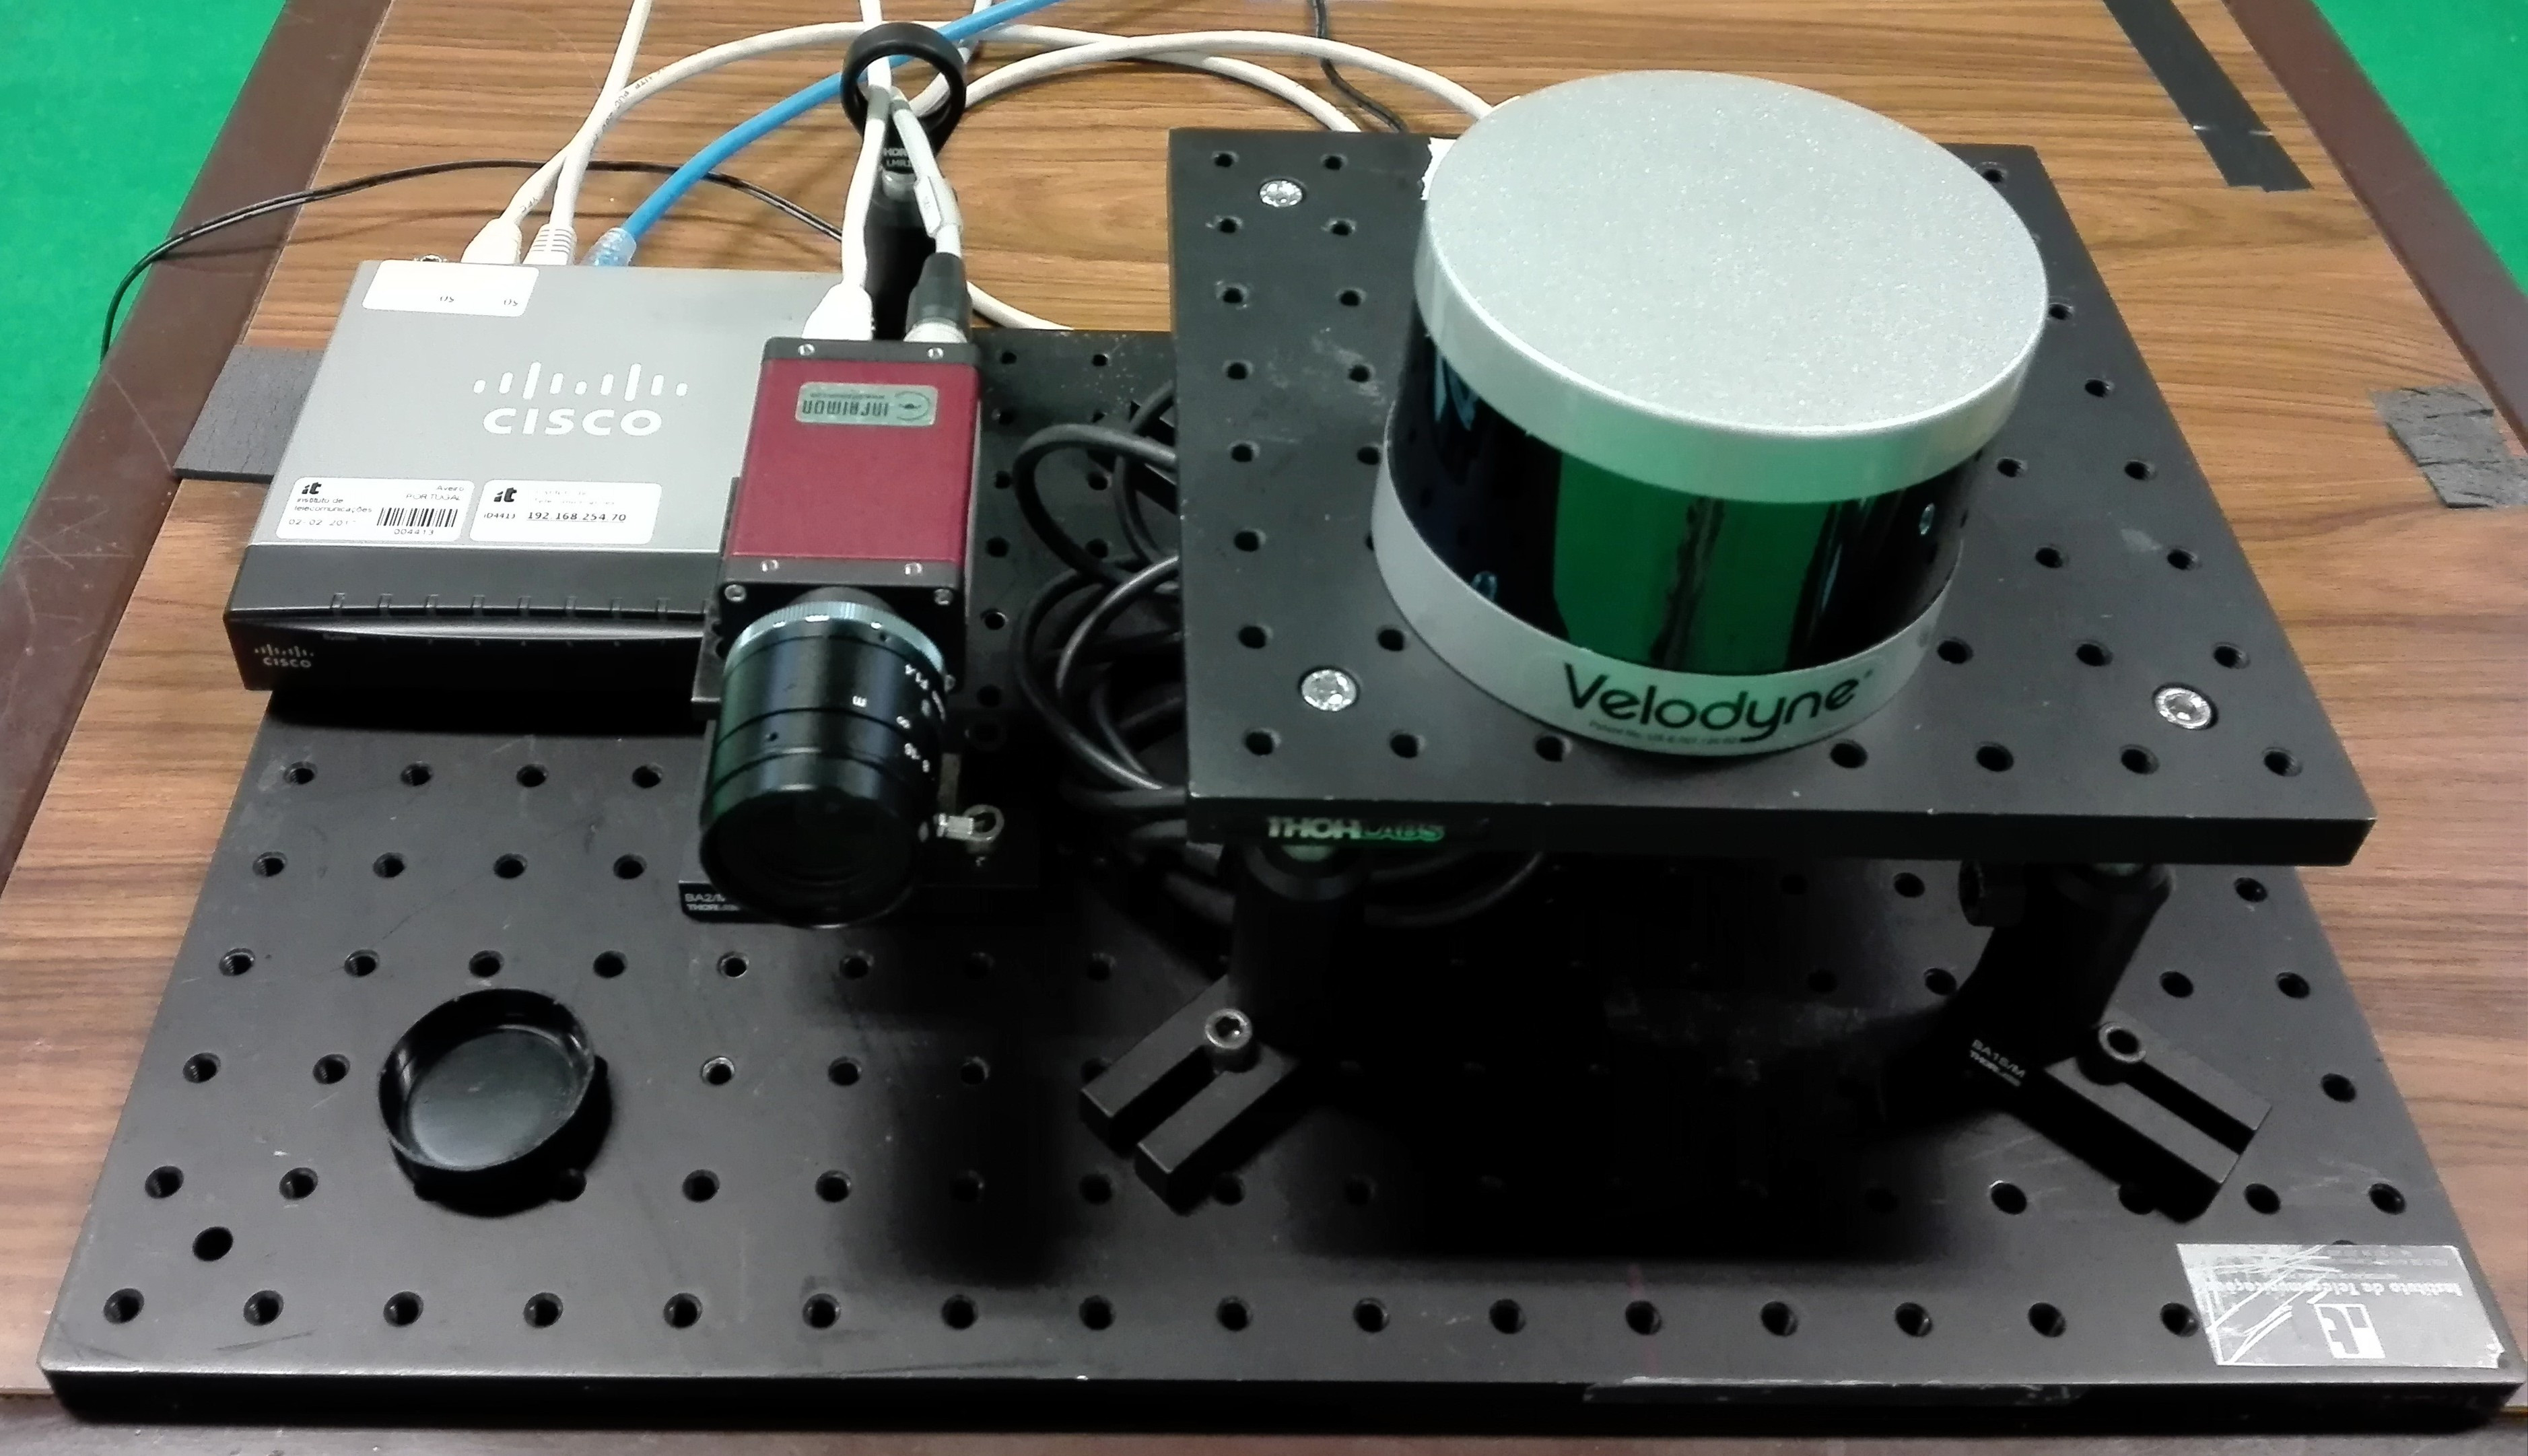
\includegraphics[width=\textwidth]{img/experimental-setup/table-setup-cambada-perspective.jpg}
		\caption{}
		\label{fig:experimental-setup:perspective}
	\end{subfigure}
	\qquad
	\begin{subfigure}[c]{0.45\textwidth}
		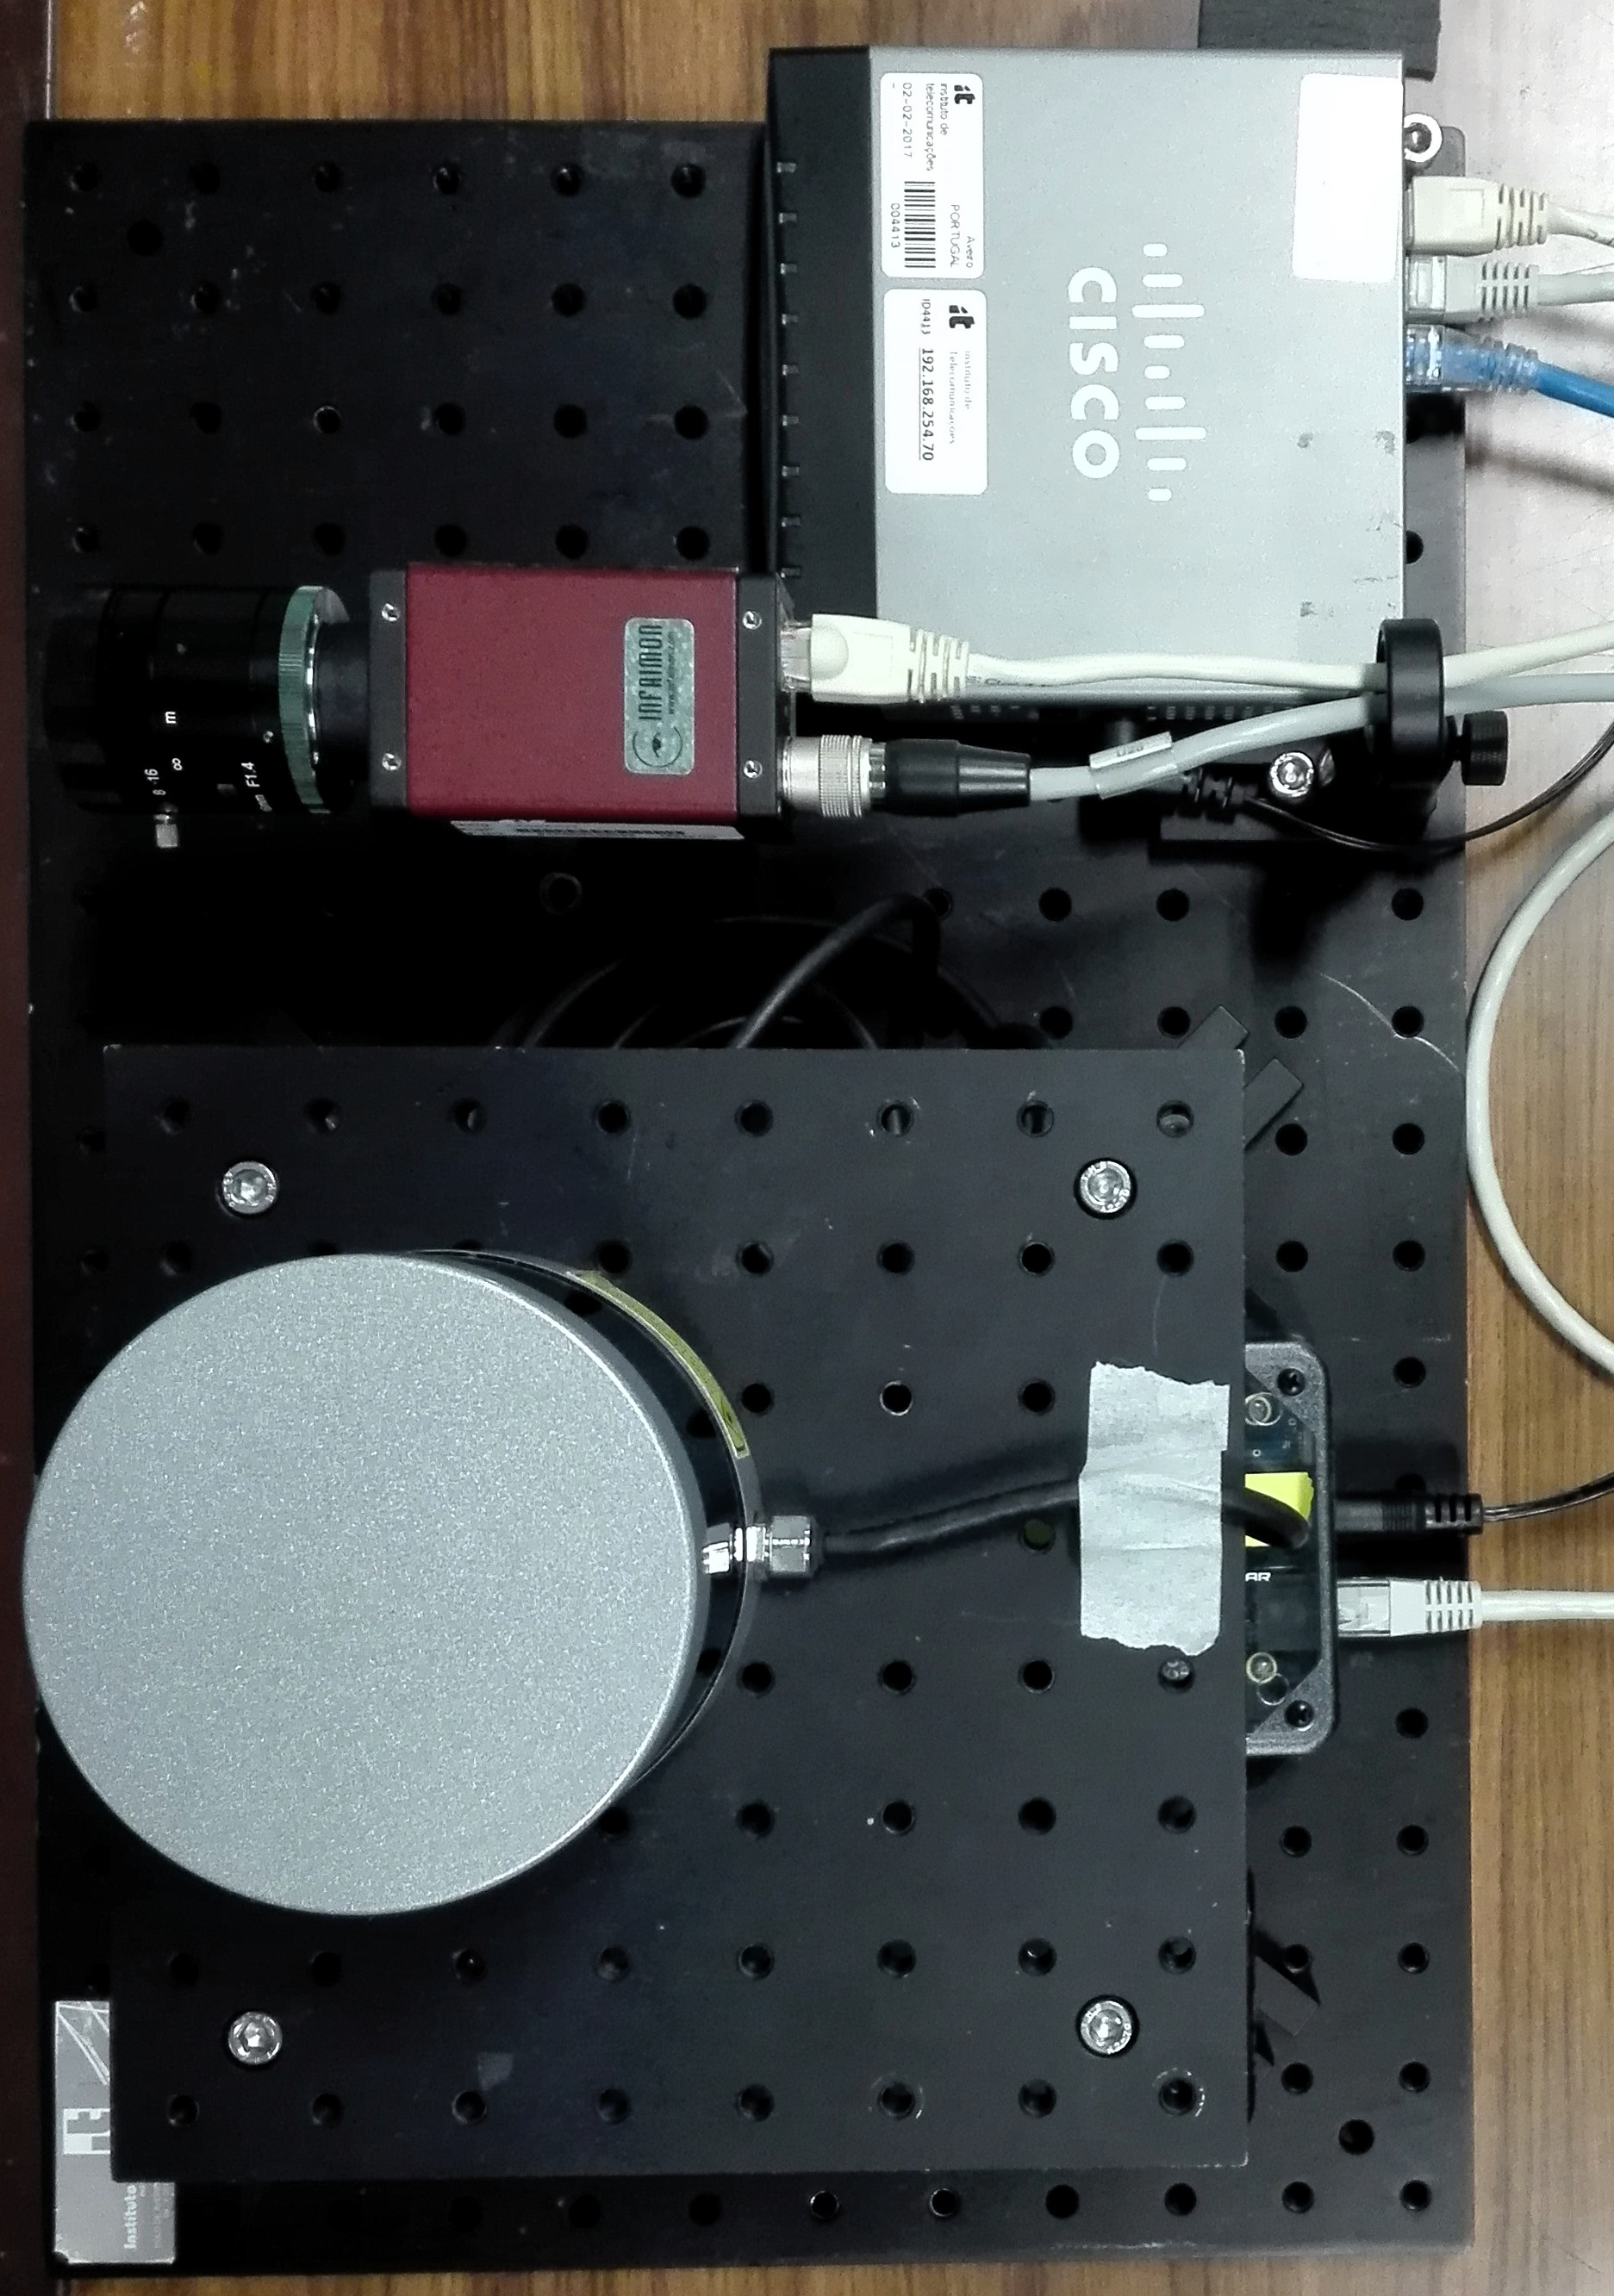
\includegraphics[width=0.65\textwidth, keepaspectratio, angle=90]{img/experimental-setup/table-setup-cambada-birds-eye.jpg}
		\caption{}
		\label{fig:experimental-setup:birds-eye}
	\end{subfigure}
	\caption[Perspective and top views of the experimental setup for the camera and \acs{lidar}.]{Relative positioning of the devices on the experimental. The \ac{lidar} is on an elevated platform to guarantee that the camera and Ethernet switch are not on its \ac{fov}. Sub-figures show the experimental setup viewed (\subref{fig:experimental-setup:perspective}) in perspective; (\subref{fig:experimental-setup:birds-eye}) from the top.}
	\label{fig:experimental-setup}
\end{figure}

\subsection{Camera and Lens}
The camera used is an industrial 5 \ac{mp} RGB camera, from \acf{avt}, model Manta G-504C. The objective is a C-Mount lens with lock from Thorlabs\cp, model MVL16M1. The full camera specifications can be accessed on~\cite{MantaG504C} and the full lens specifications on~\cite{Thorlabs}. Relevant specifications of the camera and lens are summarized  on Table~\ref{tab:camera-and-lens-specs}. 

\begin{table}[!ht]
	\renewcommand{\arraystretch}{1.2}
	\centering
	\begin{tabular}{@{}lp{7cm}l@{}}
		\toprule
		\multicolumn{2}{l}{Specification} & Value \\ \midrule
		\multicolumn{2}{l}{\emph{Camera}} & \\
		\phantom{a} & Full Resolution (width vs height) & $2452 \times 2056$ pixels \\
									& Shutter mode & Global \\
									&	Maximum \ac{fps} at full resolution & $9.2$ \\ 
									& \acs{adc}\footnotemark bit depth & $12$ bit \\\midrule 
									\multicolumn{2}{l}{\emph{Lens}} \\
									&	Focal Length & $16$ mm \\
									&	Max aperture & $f/1.4$ \\
									&	Minimum Object Distance & $300$ mm  \\
		\bottomrule
	\end{tabular}
	\caption[Relevant specifications of the camera and its lens.]{Relevant specifications for \ac{avt} Manta G-504C RGB camera (from~\cite{MantaG504C})  and MVL16M1 Thorlabs\cp~lens (from~\cite{Thorlabs}).}
	\label{tab:camera-and-lens-specs}
\end{table}

\footnotetext{\acs{adc} stands for \acl{adc}}

To power the Manta G-504C, a benchtop power source was used. Further details about powering the camera and its electrical connections are presented on Appendix-B~\ref{sec:appendix-b}.

\subsection{\ac{tof} \ac{lidar}}
The \ac{tof} \ac{lidar} used is a Velodyne VLP-16\texttrademark, a 16 beam \ac{lidar} that operates with a wavelength of \SI{903}{\nano\meter}. VLP-16 supports various measurements modes based on the return pulse (Strongest, Last, Dual) and can be connected to a \ac{gps} receiver for geopositioning and synchronization with an external clock. It also supports several rotation speeds, from 300 to 1200 \ac{rpm}, which result in different angular steps and point cloud refresh rate. The full specifications can be accessed on~\cite{VLP16} and the relevant specifications for this work are summarized on Table~\ref{tab:vlp16-specs}.

\begin{table}[!ht]
	\renewcommand{\arraystretch}{1.2}
	\centering
	\begin{tabular}{@{}p{8.3cm}l@{}}
		\toprule
		Specification & Value \\ \midrule
		Wavelength    & \SI{903}{\nano\meter} \\
		Motor \acs{rpm} & $600 \pm 3$ \\
		Angular step & \SI{0.2}{\degree} \\
		Vertical \ac{fov} & \SI{30}{\degree} \\
		Horizontal \ac{fov} & \SI{360}{\degree} \\
		Maximum Scanning Distance & \SI{100}{\meter} \\
		Theoretical Typical Distance Error & \SI{2}{\centi\meter} \\
		\bottomrule
	\end{tabular}
	\caption[Velodyne\cp~VLP-16 relevant\texttrademark relevant specifications.]{Velodyne VLP-16 relevant specifications. Source~\cite{VLP16}.}
	\label{tab:vlp16-specs}
\end{table}


\subsection{Connection Setup} 
Both Velodyne VLP-16 and \ac{avt} Manta G-504C operate over Gigabit Ethernet. Therefore, a Gigabit  Ethernet switch is required to connect all the equipment to a single computer using a single Ethernet port. The switch used was Cisco SG200-08, an 8-Port Gigabit Smart Switch. 

The switch was configured so that every port was on the same \ac{vlan}, ensuring packets were accessible on the computer, since the sensors were configured to broadcast the packets. An alternative to this implementation was to redirect the packets from each sensor to the computer network and filter the packets from the computer to the sensors, by putting them on separated networks and create a network traffic management solution. Using \ac{ros} capabilities to measure packet delay and rate of publishing of the data messages, no bandwidth constraints or packet delay/loss were verified. Therefore, the solution chosen was the former, due to its simplicity. 

For each device a fixed \acf{ip} address was attributed, following the instructions on their datasheet~\cite{VLP16, MantaVision2013}. The \ac{ip} addresses can be consulted on Table~\ref{tab:experimental-setup-ip}.

\begin{table}[!ht]
	\renewcommand{\arraystretch}{1.2}
	\centering
	\begin{tabular}{@{}lcc@{}}
		\toprule
		Device          & \ac{ip} Address & Subnet Mask\\ \midrule
		Computer        & 192.168.10.77  & 255.255.255.0 \\
		Manta G-504C    & 192.168.10.1   & 255.255.255.0 \\
		Velodyne VLP-16 & 192.168.10.201 & 255.255.255.0 \\
		\bottomrule
	\end{tabular}
	\caption[\acs{ip} addresses and subnet masks for the devices connected on the experimental setup.]{\ac{ip} addresses and subnet masks for the devices connected on the experimental setup.}
	\label{tab:experimental-setup-ip}
\end{table}

\subsection{\ac{lidar} and Camera Interference}
No significant interference is expected between the camera and the \ac{lidar}. Despite the camera lens having a transmission coefficient of $66\%$ at $\approx 900 nm$~\cite{Thorlabs}, and Sony ICX655, the camera sensor for the \ac{avt} Manta G-504C, having a Quantum Efficiency of $\approx 5\%$~\cite{MantaG504C}, \ac{avt} Manta G-504C is equipped with an \ac{ir} cut-filter.

Despite the low sensibility of the camera and the presence of an \ac{ir} cut-filter, an experiment was conducted to verify the occurrence of interference. The experimental setup was switched on in a Dark Room without any other light sources and the camera feed was visualized. Besides the noise caused by the camera electronics operation, no signs of interference caused by the \ac{lidar} infrared beams could be observed on the camera image feed, since no bright spots were found. Therefore, no further work on \ac{lidar} to camera interference were carried


%\begin{figure}[H]
%	\centering
%	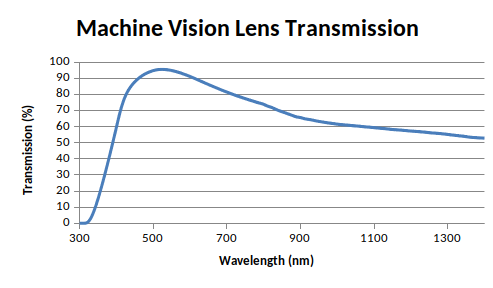
\includegraphics[width=0.6\textwidth]{img/experimental-setup/lens-transmission.png}
%	\caption{Transmission of the MVL16M1 lens in relation the light wavelength. Source~\cite{Thorlabs}}
%	\label{fig:lens-transmission}
%\end{figure}



\section{Camera Intrinsic Calibration}
\label{sec:calibration:camera}
The act of calibrating a camera consists on determining its intrinsic parameters, as detailed in sub-Section~\ref{subsec:sota:camera-intrinisc-calibration}. This can be done by taking different images with a known pattern, fully visible on the camera \ac{fov}, changing its rotation and translation in relation to the camera coordinate frame.

The calibration procedure undertaken uses a chessboard of $13 \times 9$ squares, with each square having an edge length of \SI{44.0}{\milli\meter}. The chessboard used can be seen on Figure~\ref{fig:chessboard}. It was laser printed on a \SI{100}{\gram} A2 paper and then glued to a plywood board.

\begin{figure}[H]
	\centering
	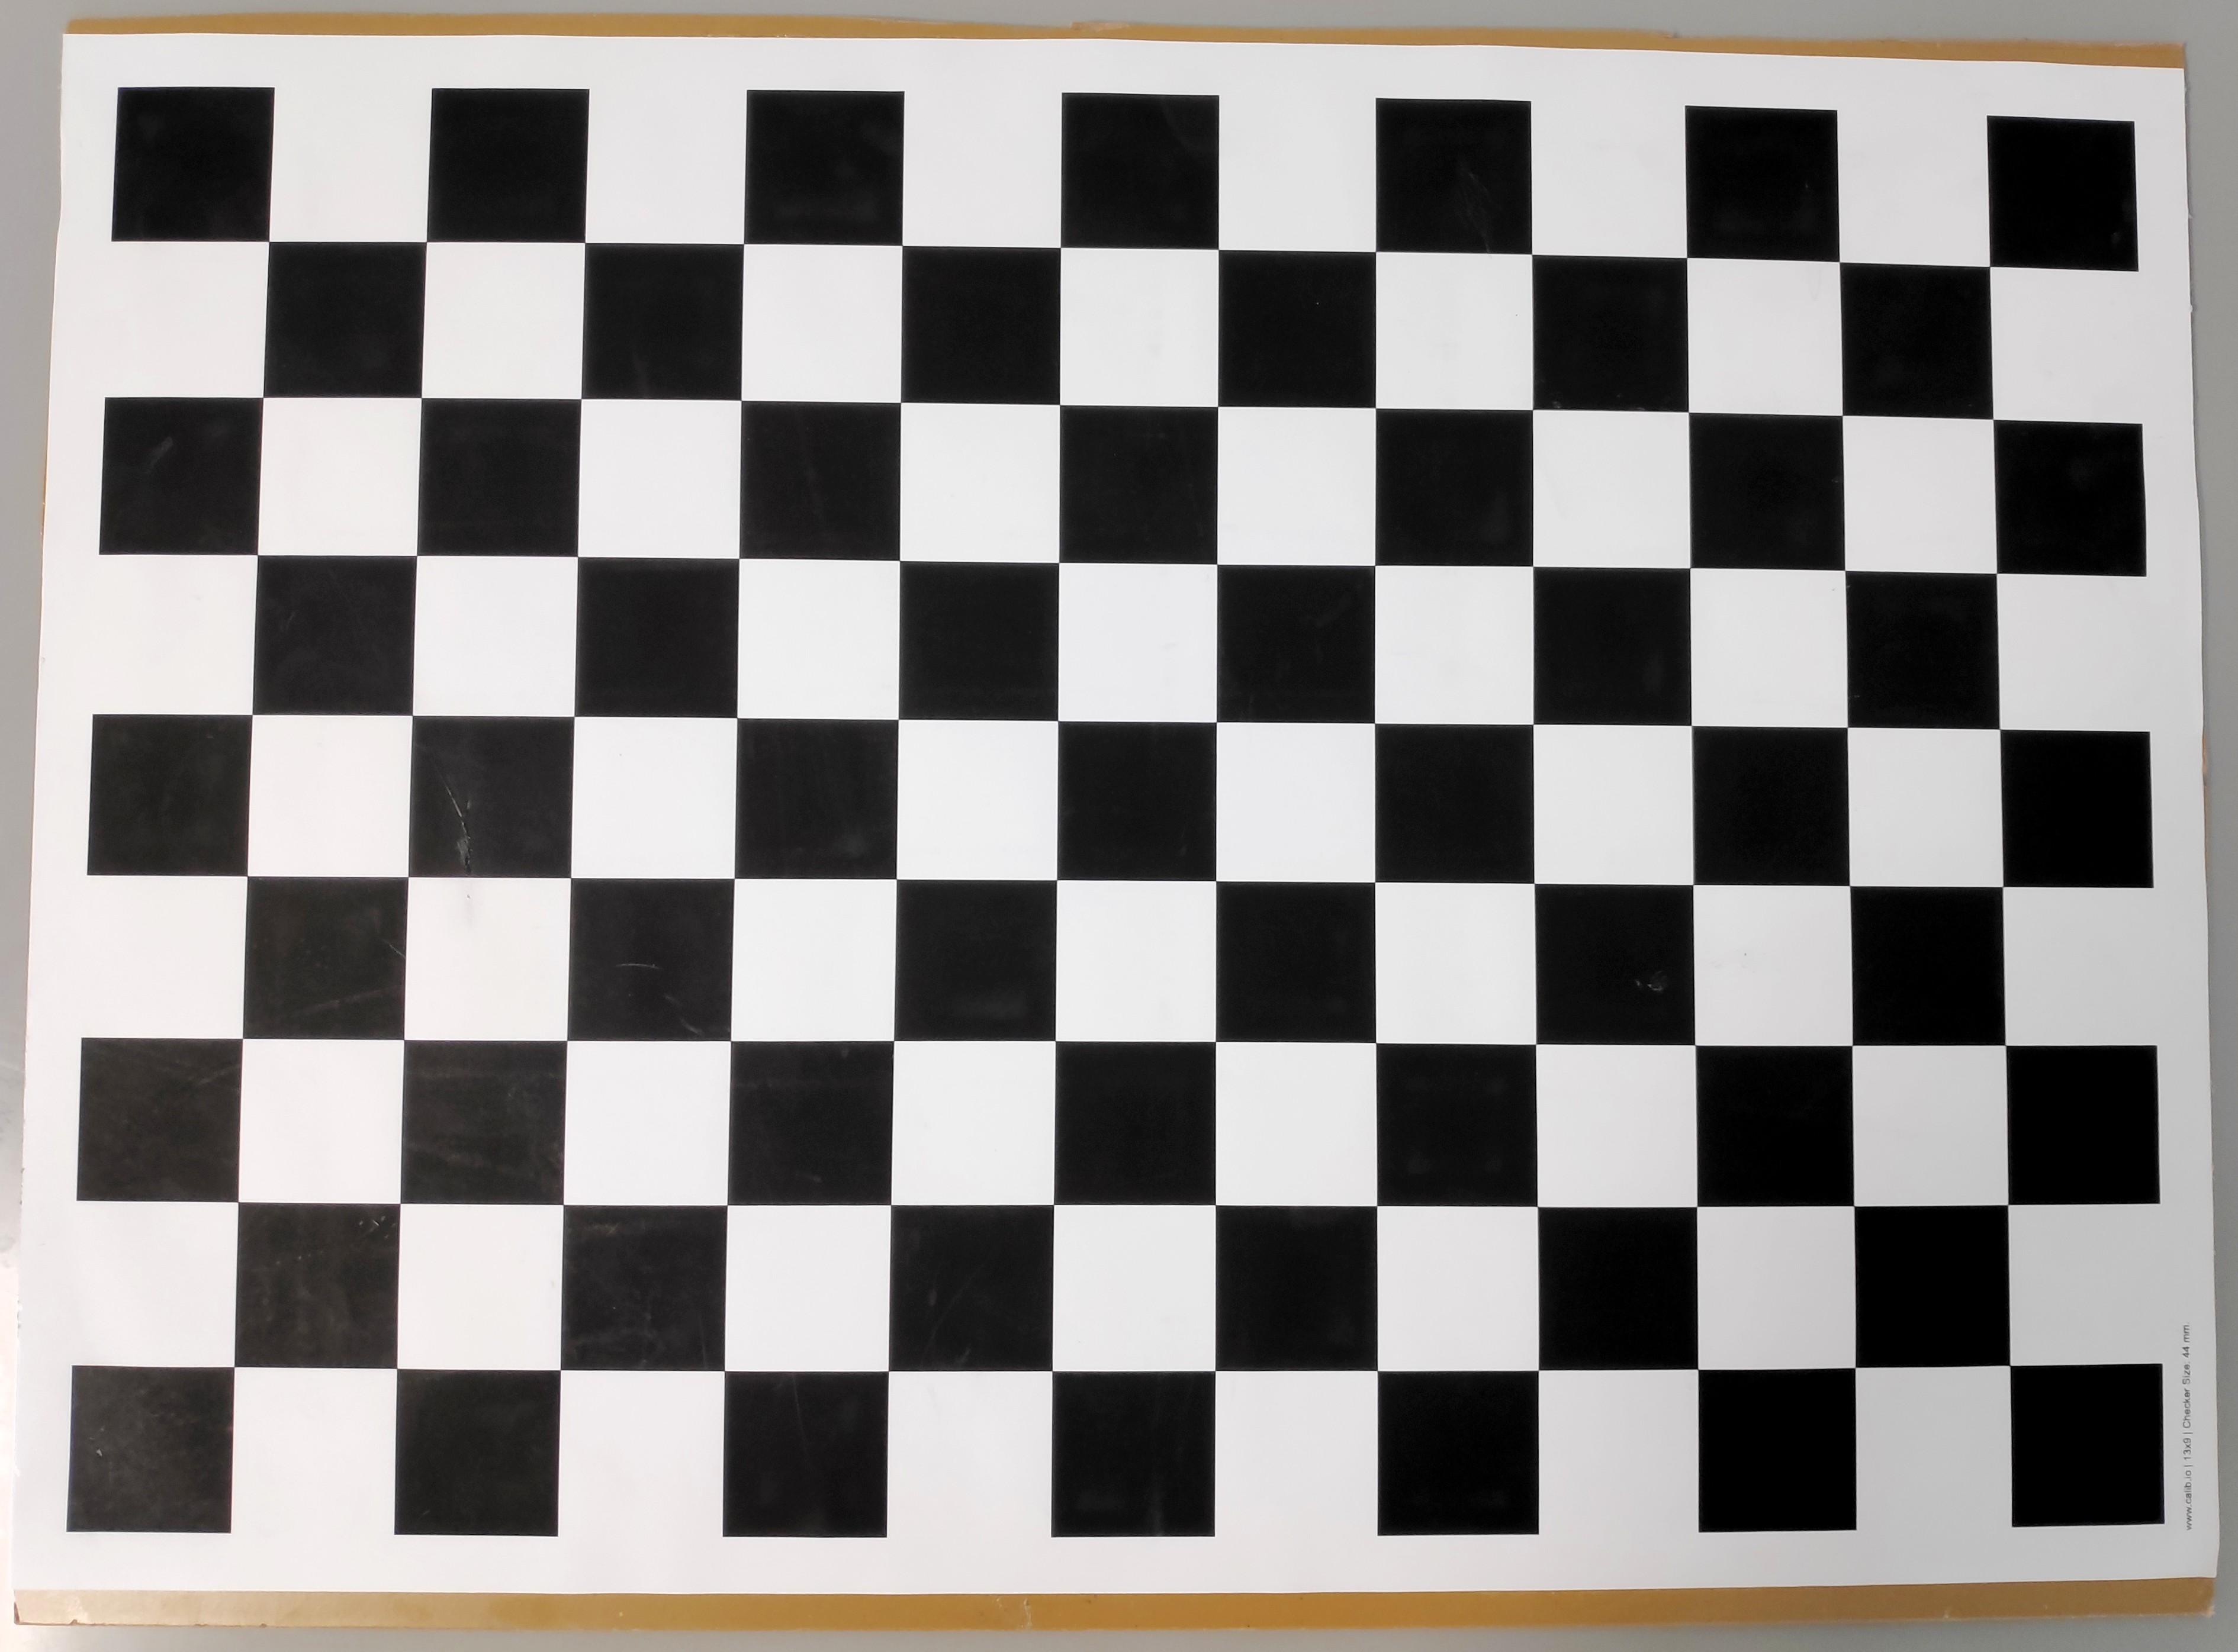
\includegraphics[width=0.5\textwidth]{img/experimental-setup/chessboard.jpg}
	\caption{Chessboard used during camera calibration procedures. The chessboard was laser printed on A2 paper size, in real size, that was then glued to a plywood board.}
	\label{fig:chessboard}
\end{figure}

Calibrating the camera requires that the calibration object to be focused. Therefore, before any proper calibration can be made, focus theory and procedure are given on the next sub-section,~\ref{subsec:calibration:camera-focus}.


\subsection{Camera Focus and \acl{dof}}
\label{subsec:calibration:camera-focus}
Focusing a camera can only be attained for an exact distance from the camera~\cite{Merklinger1993, Photopillers}, measured perpendicularly to the plane of focus, which is the plane containing the \ac{cmos} or \ac{ccd} chip. Therefore, on every image, there is a plane of focus and what actually ``looks focused'' is really just in ``acceptably sharp focus''.

``Acceptably sharp focus'' means that a point in the real world would not result in a point on the image (as happens in precise focus), but in a blurred spot~\cite{Photopillers}. However, if the size of blur is small enough, little to no differences can be perceived and the image is considered to be focused~\cite{Photopillers}. The maximum size at which this blur is not noticed by the viewer (given a specific sensor size, dimension of the viewed photo, viewing distance and acuity of the viewer) is when the \ac{coc} is smaller than the pixel size~\cite{Photopillers, Merklinger1993}.

The first step in focusing an image requires the calculation of the hyperfocal distance, $H$, the distance at which the camera is focused to ensure objects from half of this distance to the infinity are in an ``acceptably sharp focus'' (referred to as just focus, from now on). This distance can be calculated using the equation~\eqref{eq:hyperfocal_distance}, below, where $f$ is the focal length, $F_N$ is the F-number and $c$ the \ac{coc} limit. Hyperfocal near limit is defined as $H_\text{near} = \rfrac{H}{2}$.

\begin{equation}
	\label{eq:hyperfocal_distance}
	H = \frac{f^2}{F_Nc} + f \approx \frac{f^2}{F_Nc} 
\end{equation}

Known the hyperfocal distance, the \acf{dof} can be calculated. \ac{dof} is measured in meters and is obtained by subtracting the farthest and nearest distances at which an object is focused (see Equation~\eqref{eq:dof}), indicating the distance between this two points~\cite{Photopillers, Merklinger1993, mvg_book}. The nearest and farthest points can be calculated using the equations~\eqref{eq:dof-near} and~\eqref{eq:dof-far}, respectively, where $d$ is the target object distance to the camera sensor.

\begin{subequations}
	\label{eq:dof_all}
	\begin{align}
		DoF & = DoF_{far} - DoF_{near} \label{eq:dof} \\
		DoF_{far} & = \frac{H\times d}{H - (d - f)} \label{eq:dof-far} \\
		DoF_{near} & = \frac{H\times d}{H + (d - f)} \label{eq:dof-near} 
	\end{align}
\end{subequations}

Equations~\eqref{eq:dof_all} make it possible to select a desired \acl{dof} for an image that guarantees that all the objects of interest are focused. Taking in consideration that smaller apertures (bigger F-numbers) will increase the exposition time~\cite{Merklinger1993} (since the amount of light illuminating the sensor will be lower), a target distance can be selected with the guarantee that all the objects from the near \ac{dof} point to the far \ac{dof} will be sharp.

Rewriting the Equation~\eqref{eq:dof-near} to calculate the objects distance, giving the minimum distance at the objects must be focused, one gets: %the Equation~\eqref{eq:dof-subject-distance}.

\begin{equation}
	\label{eq:dof-subject-distance}
	d = \frac{(H - f) \cdot DoF_{near}}{H - DoF_{near}}
\end{equation}


\subsection{Camera Calibration Procedure}
For calibration, \ac{opencv} algorithms are used~\cite{opencv_doc}, such as \texttt{calibrateCamera}, \texttt{solvePnP} and \texttt{findChessboardCorners}. These algorithms, the underlying code interconnecting them and a \ac{gui} for performing calibration are available in a \ac{ros} package, \texttt{camera\_calibration} from the \texttt{image\_pipeline} metapackage~\cite{cameraCalibrationRos}, which we use for intrinsic camera calibration.

For calibration, around 50 unique photos are taken for each setup. These images are converted to greyscale, the chessboard corners are detected and the camera intrinsic parameters are computed by the \texttt{camera\_calibration} ROS package. A subset of the calibration images is presented on Figure~\ref{fig:camera-calibration-images}.

\begin{figure}[!ht]
	\centering
	\begin{subfigure}[c]{0.30\textwidth}
		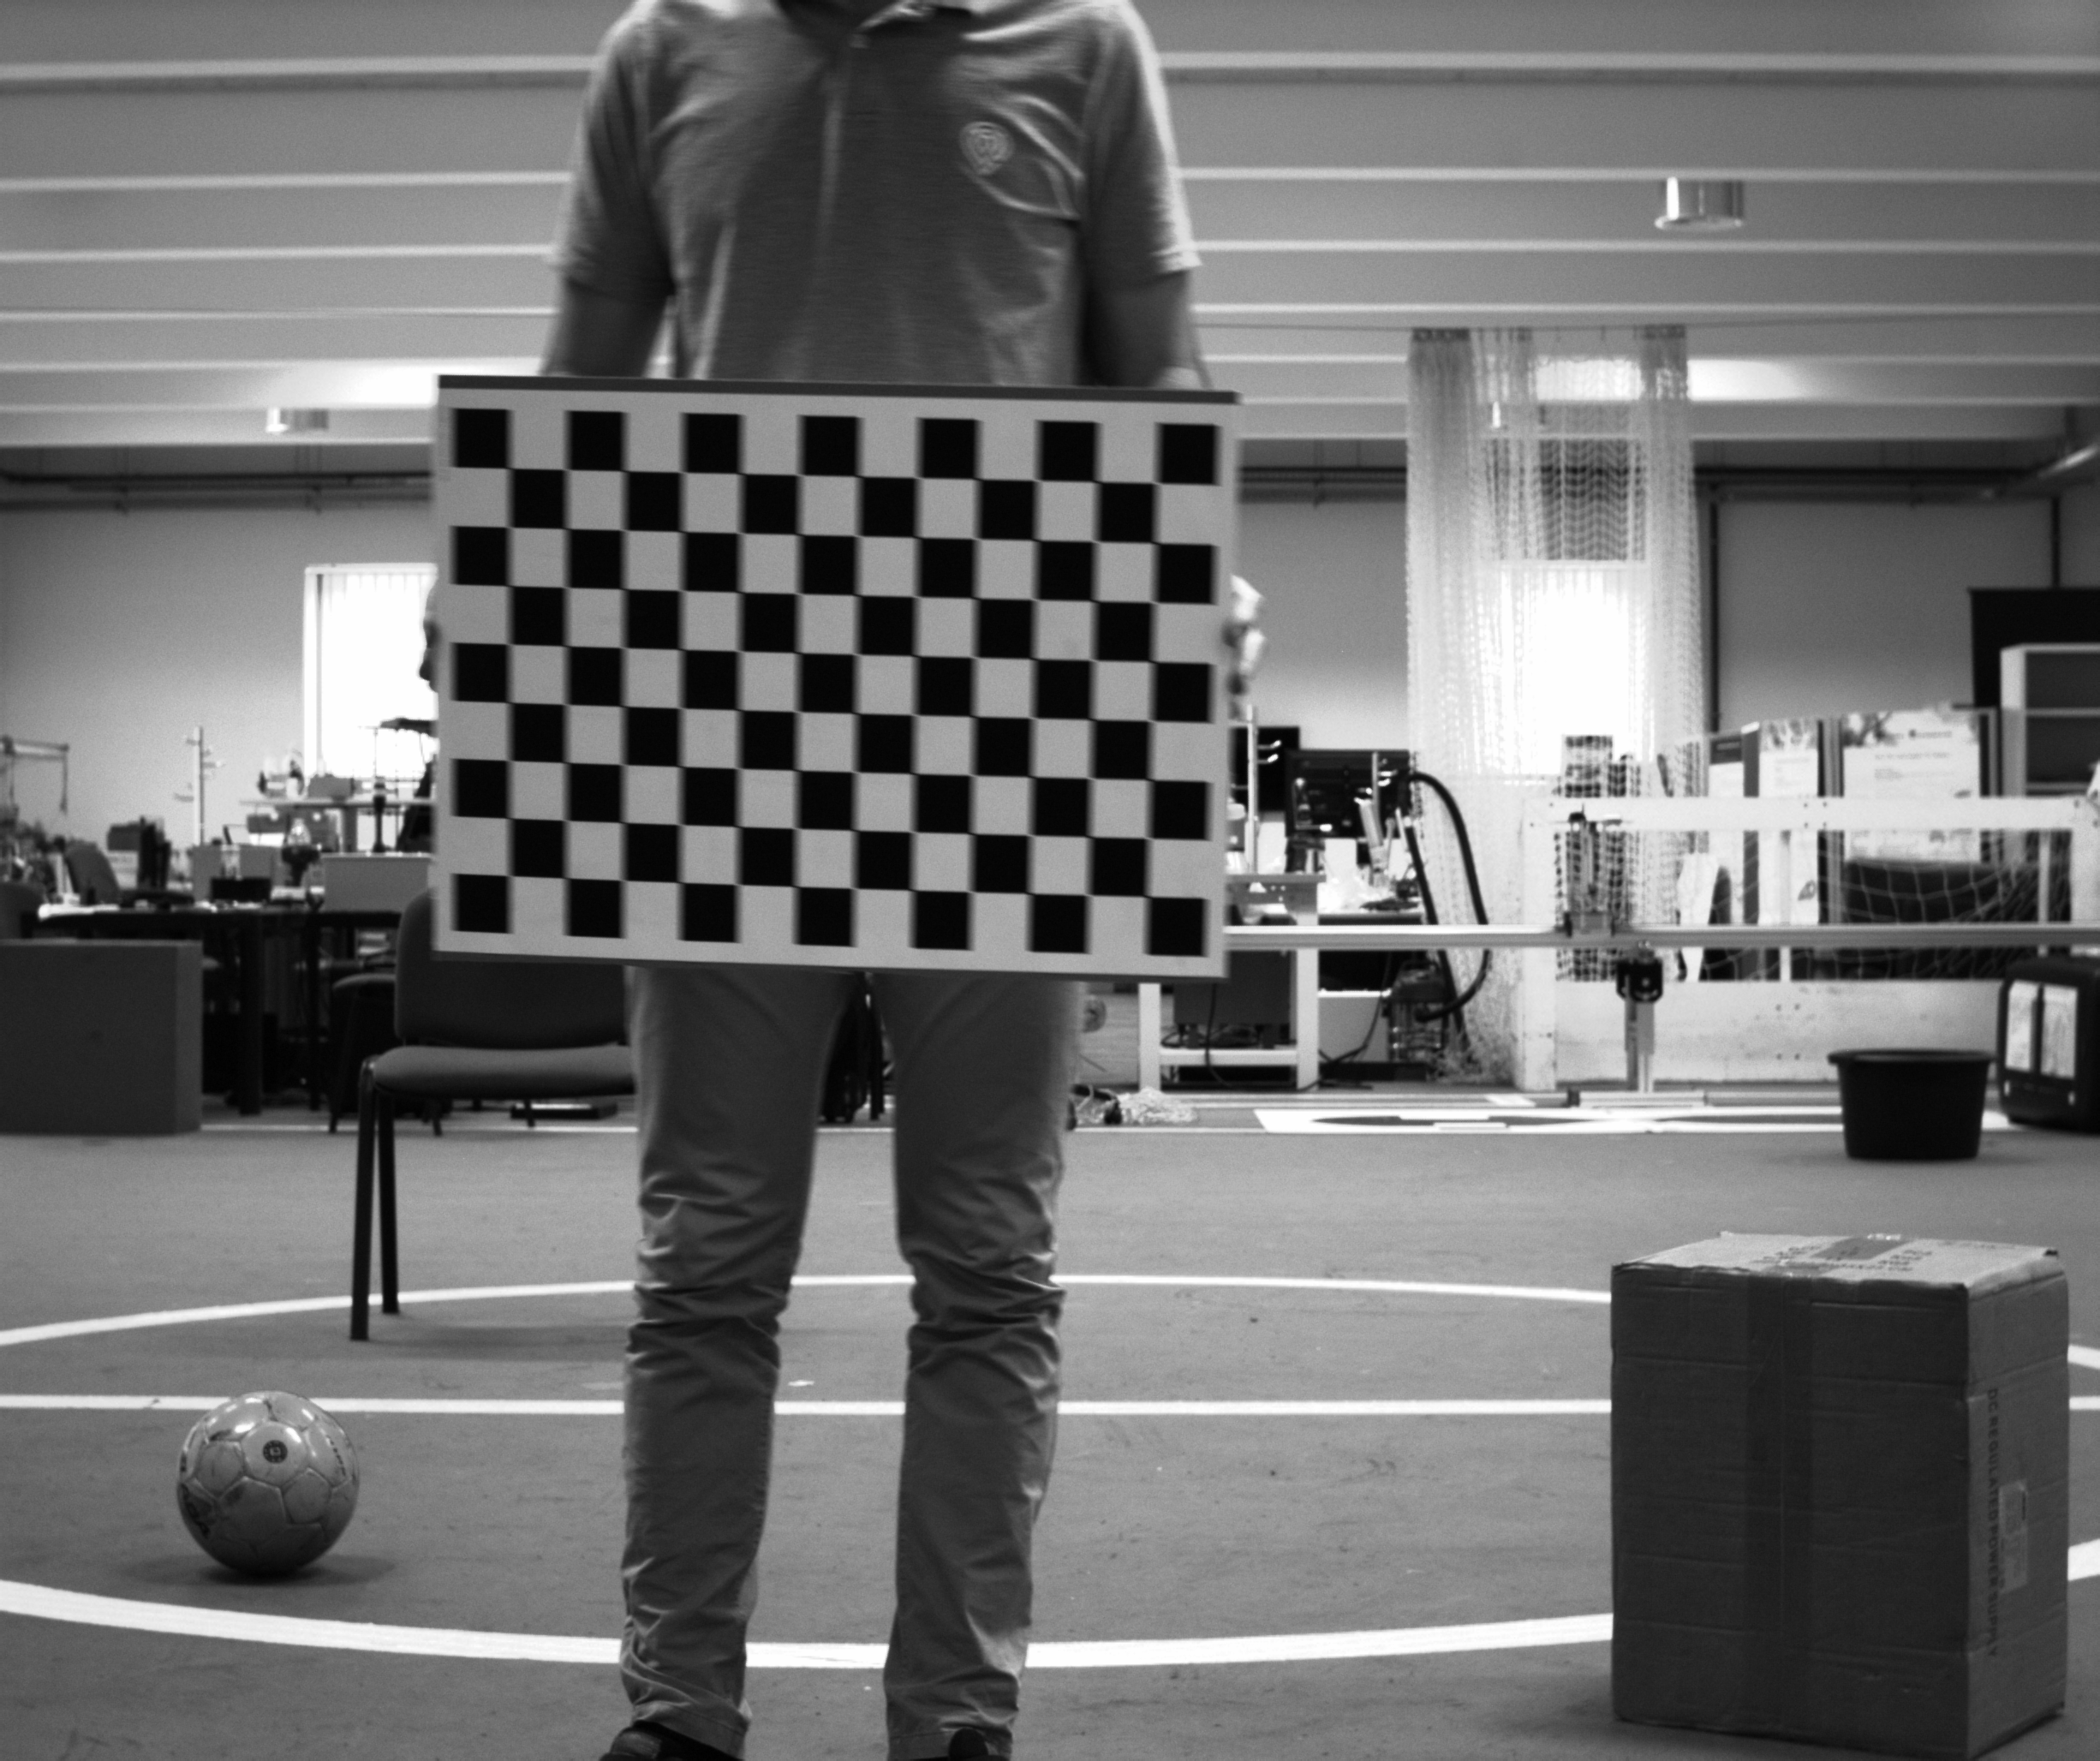
\includegraphics[width=0.9\textwidth]{img/camera-calibration/left-0001.png}
	\end{subfigure}
	\begin{subfigure}[c]{0.30\textwidth}
		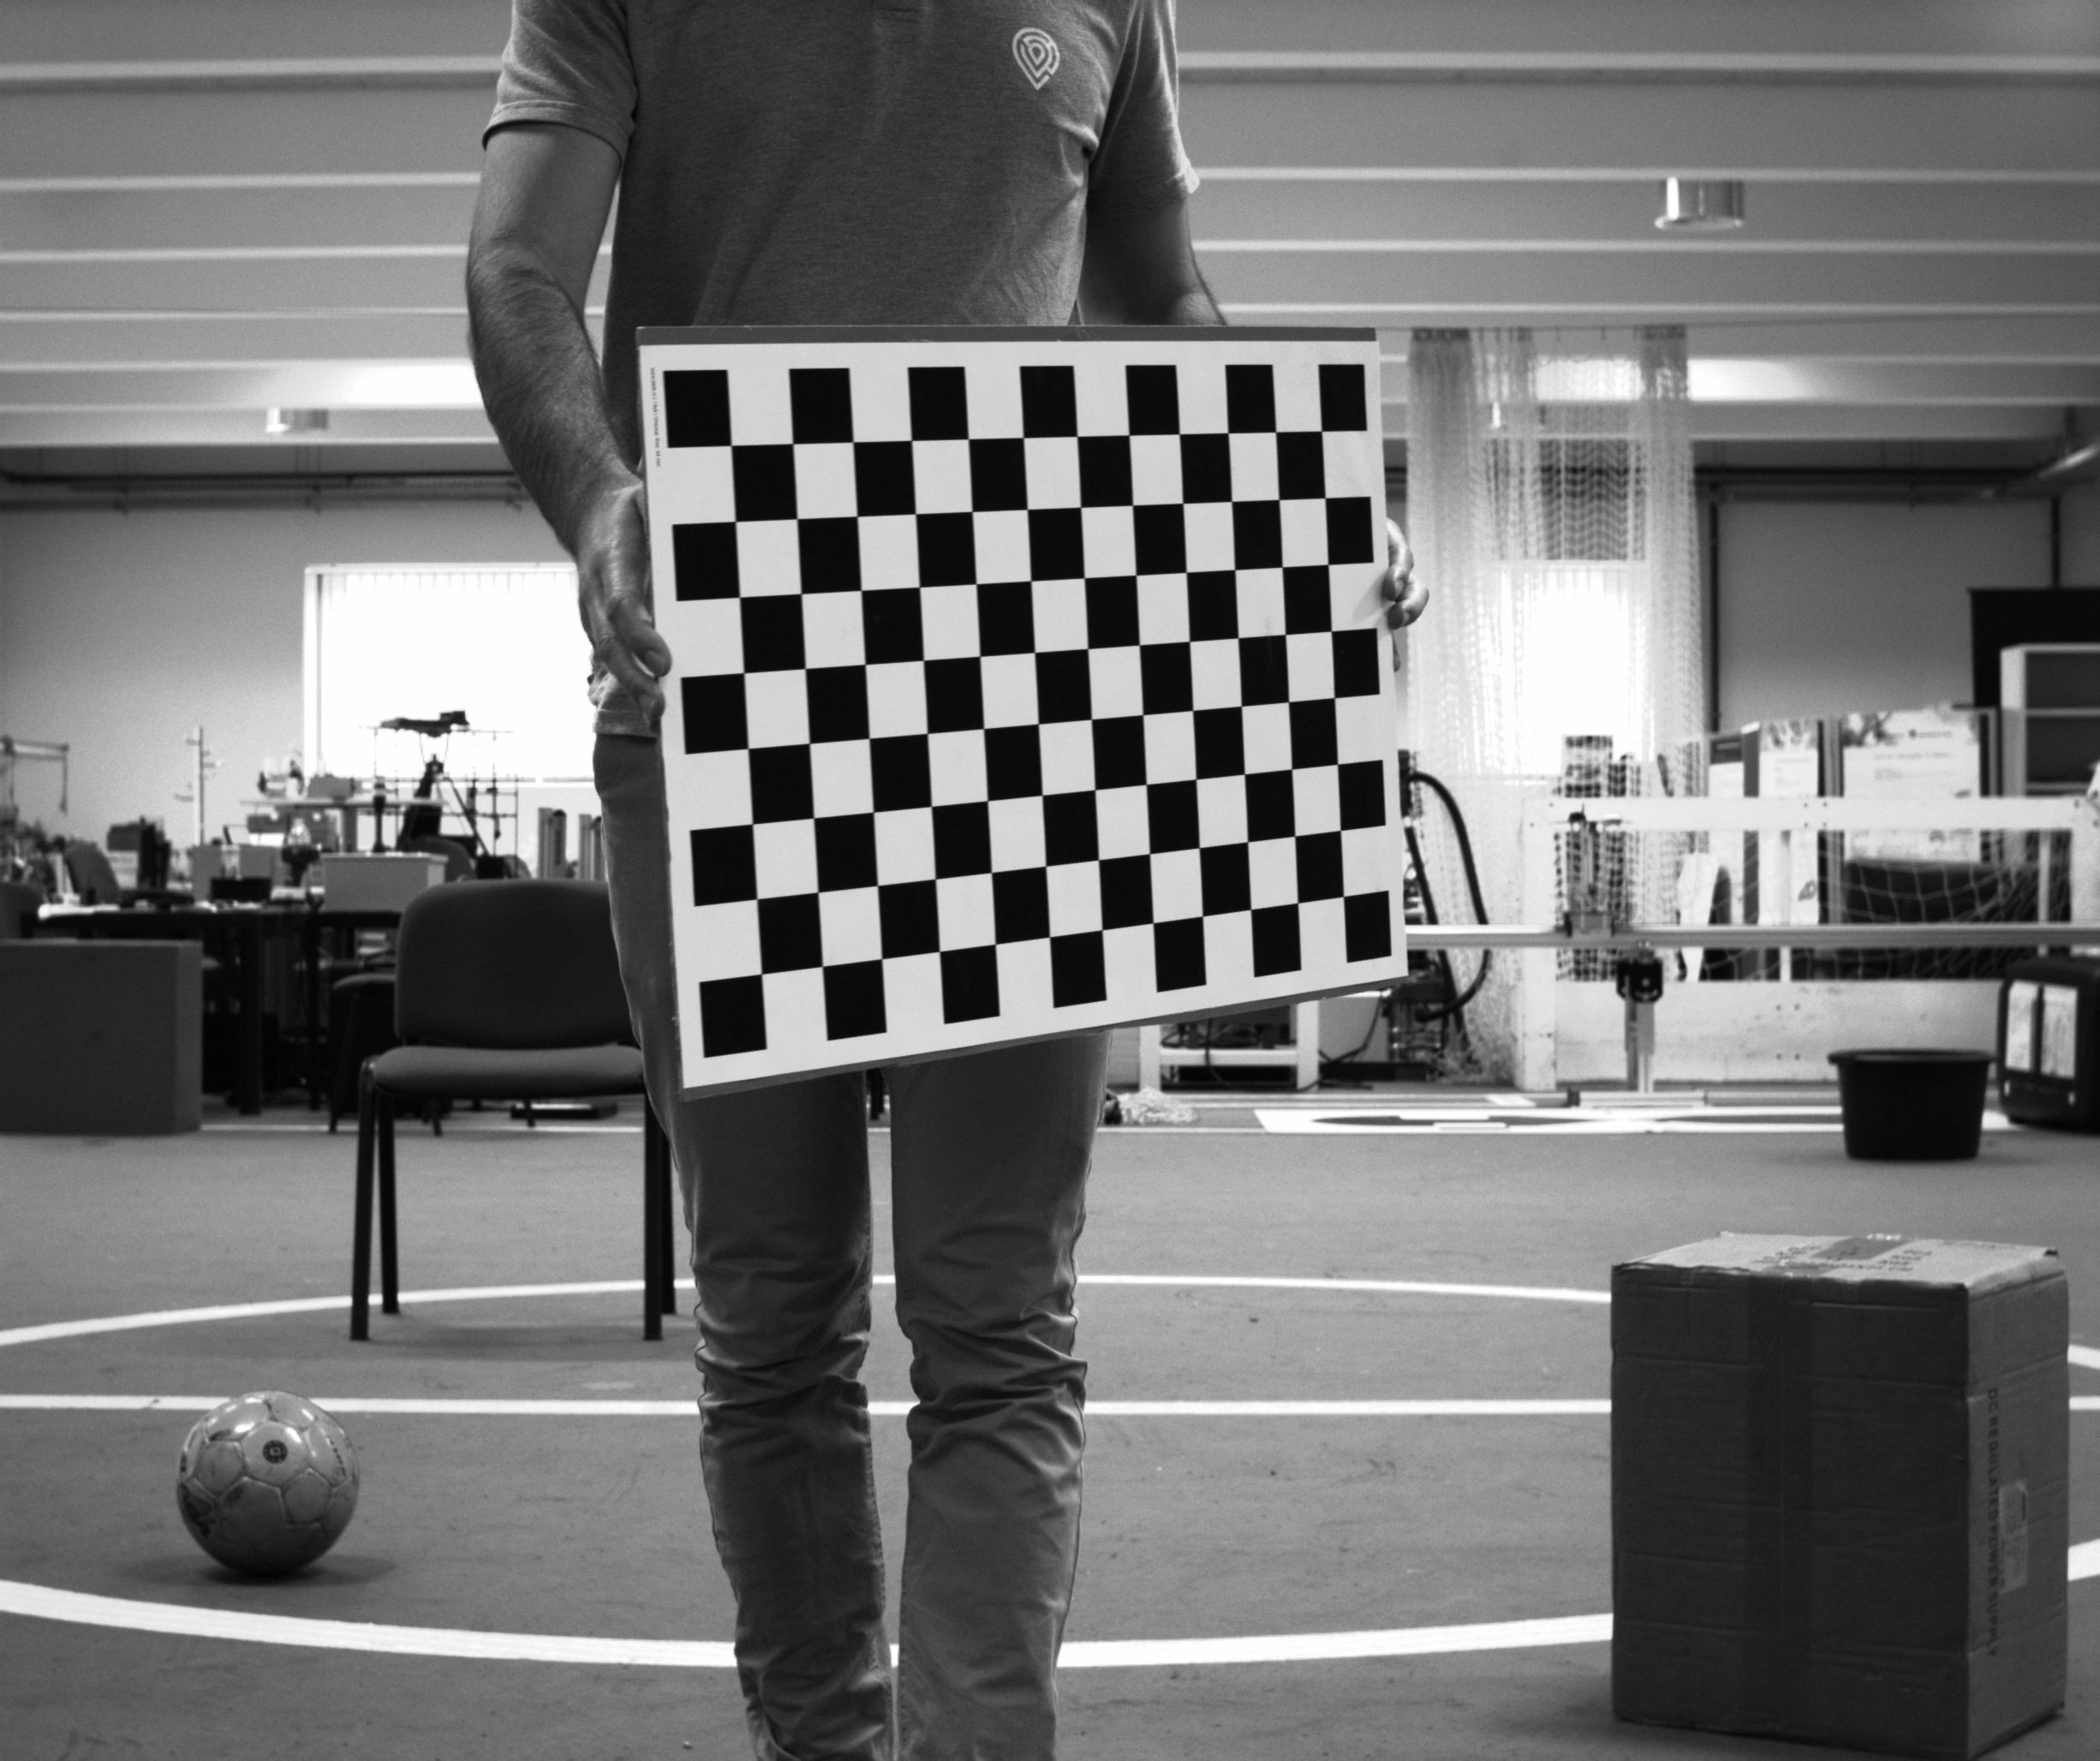
\includegraphics[width=0.9\textwidth]{img/camera-calibration/left-0005.png}
	\end{subfigure}
	\begin{subfigure}[c]{0.30\textwidth}
		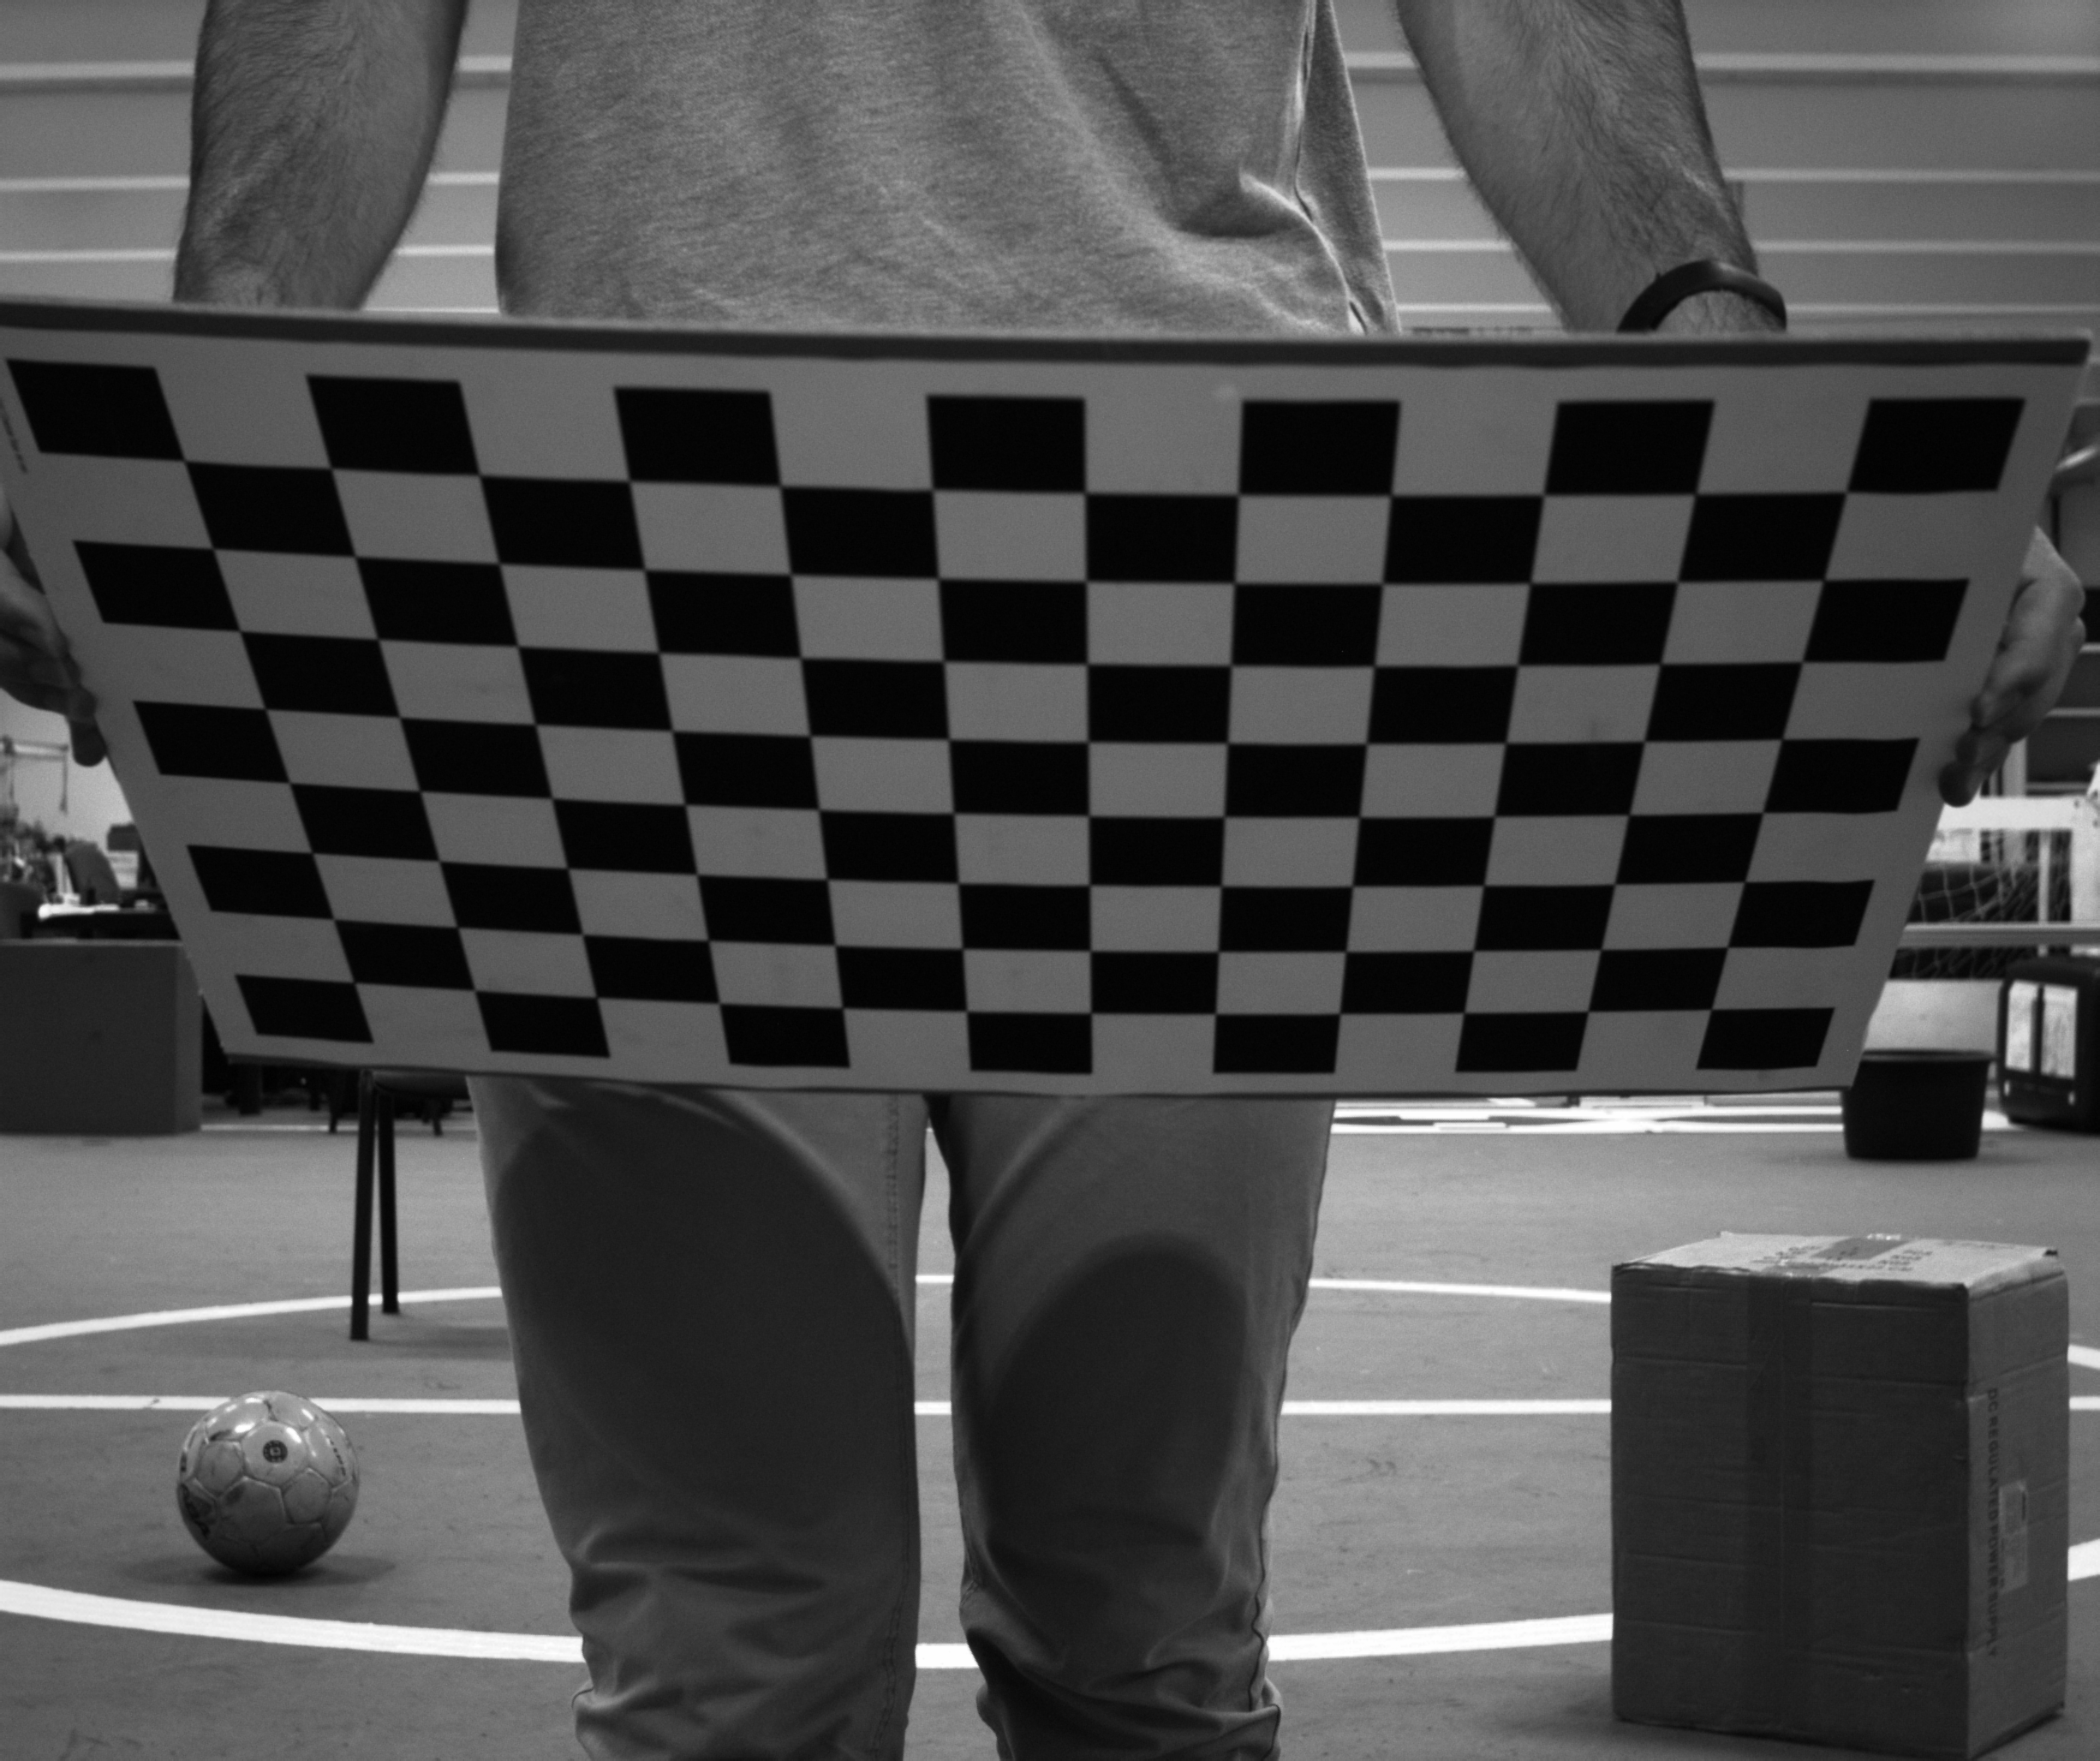
\includegraphics[width=0.9\textwidth]{img/camera-calibration/left-0022.png}
	\end{subfigure}
	\\ 
	\vspace{5mm}
	\begin{subfigure}[c]{0.30\textwidth}
		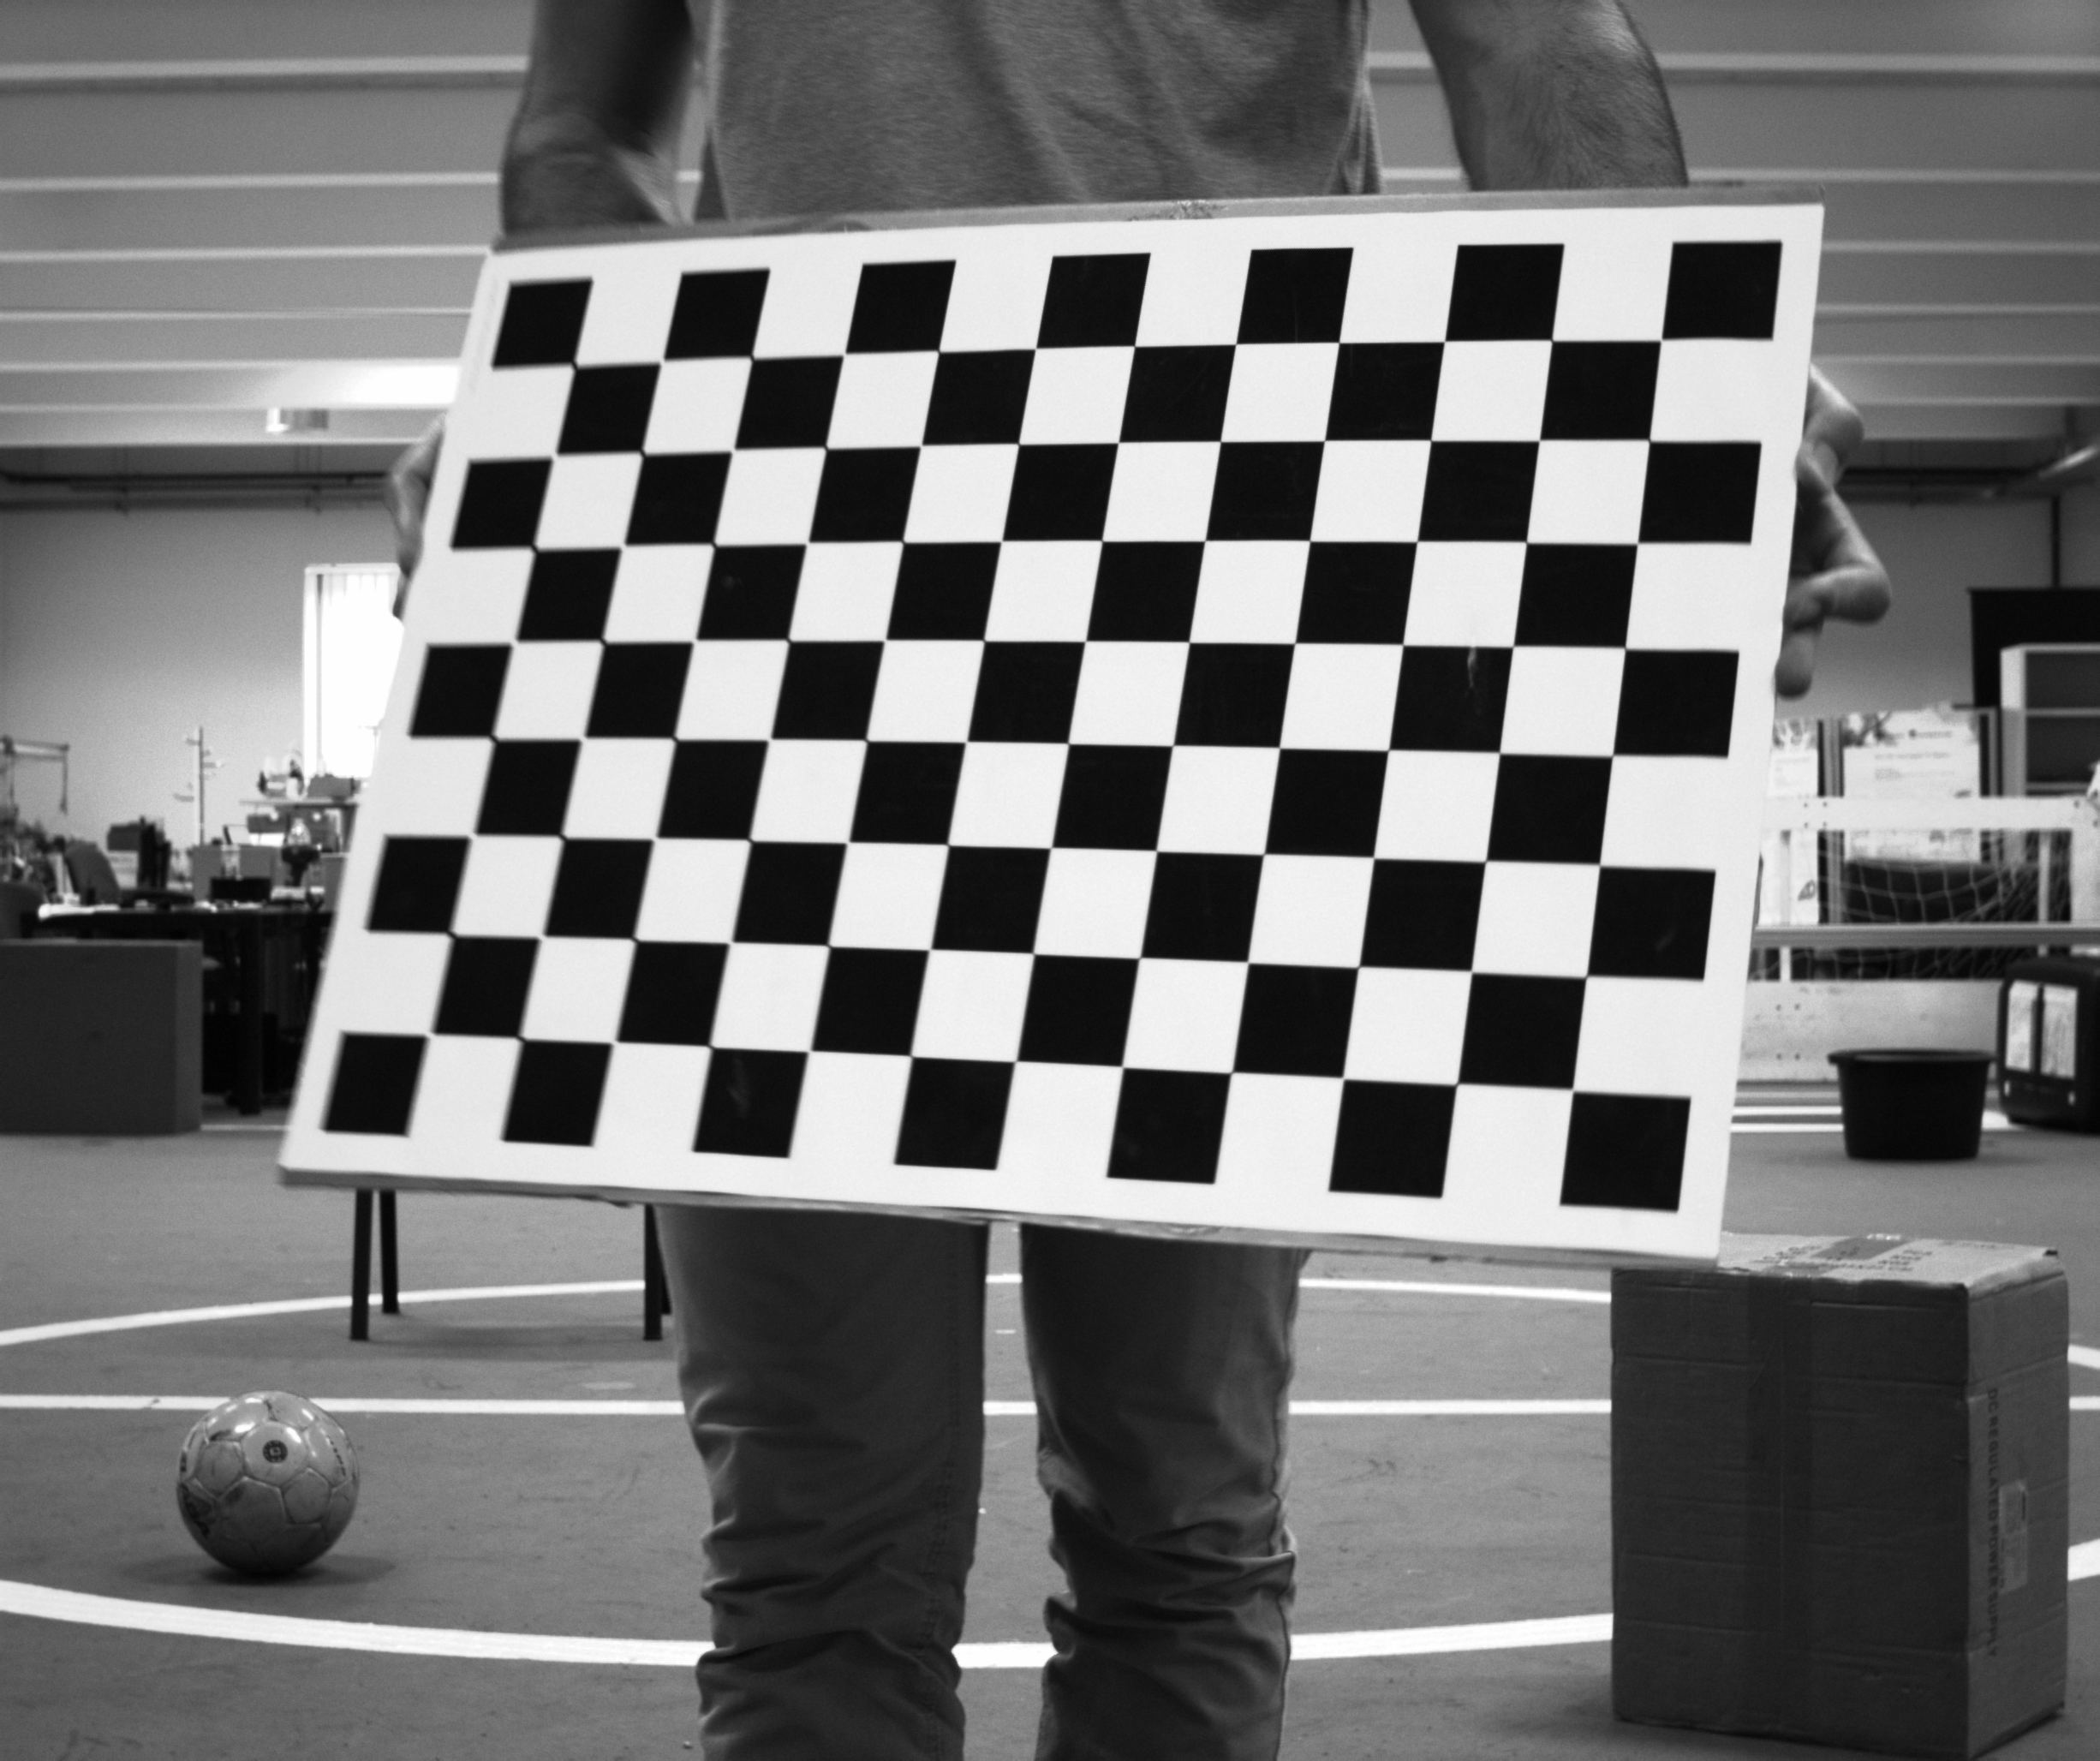
\includegraphics[width=0.9\textwidth]{img/camera-calibration/left-0030.png}
	\end{subfigure}
	\begin{subfigure}[c]{0.30\textwidth}
		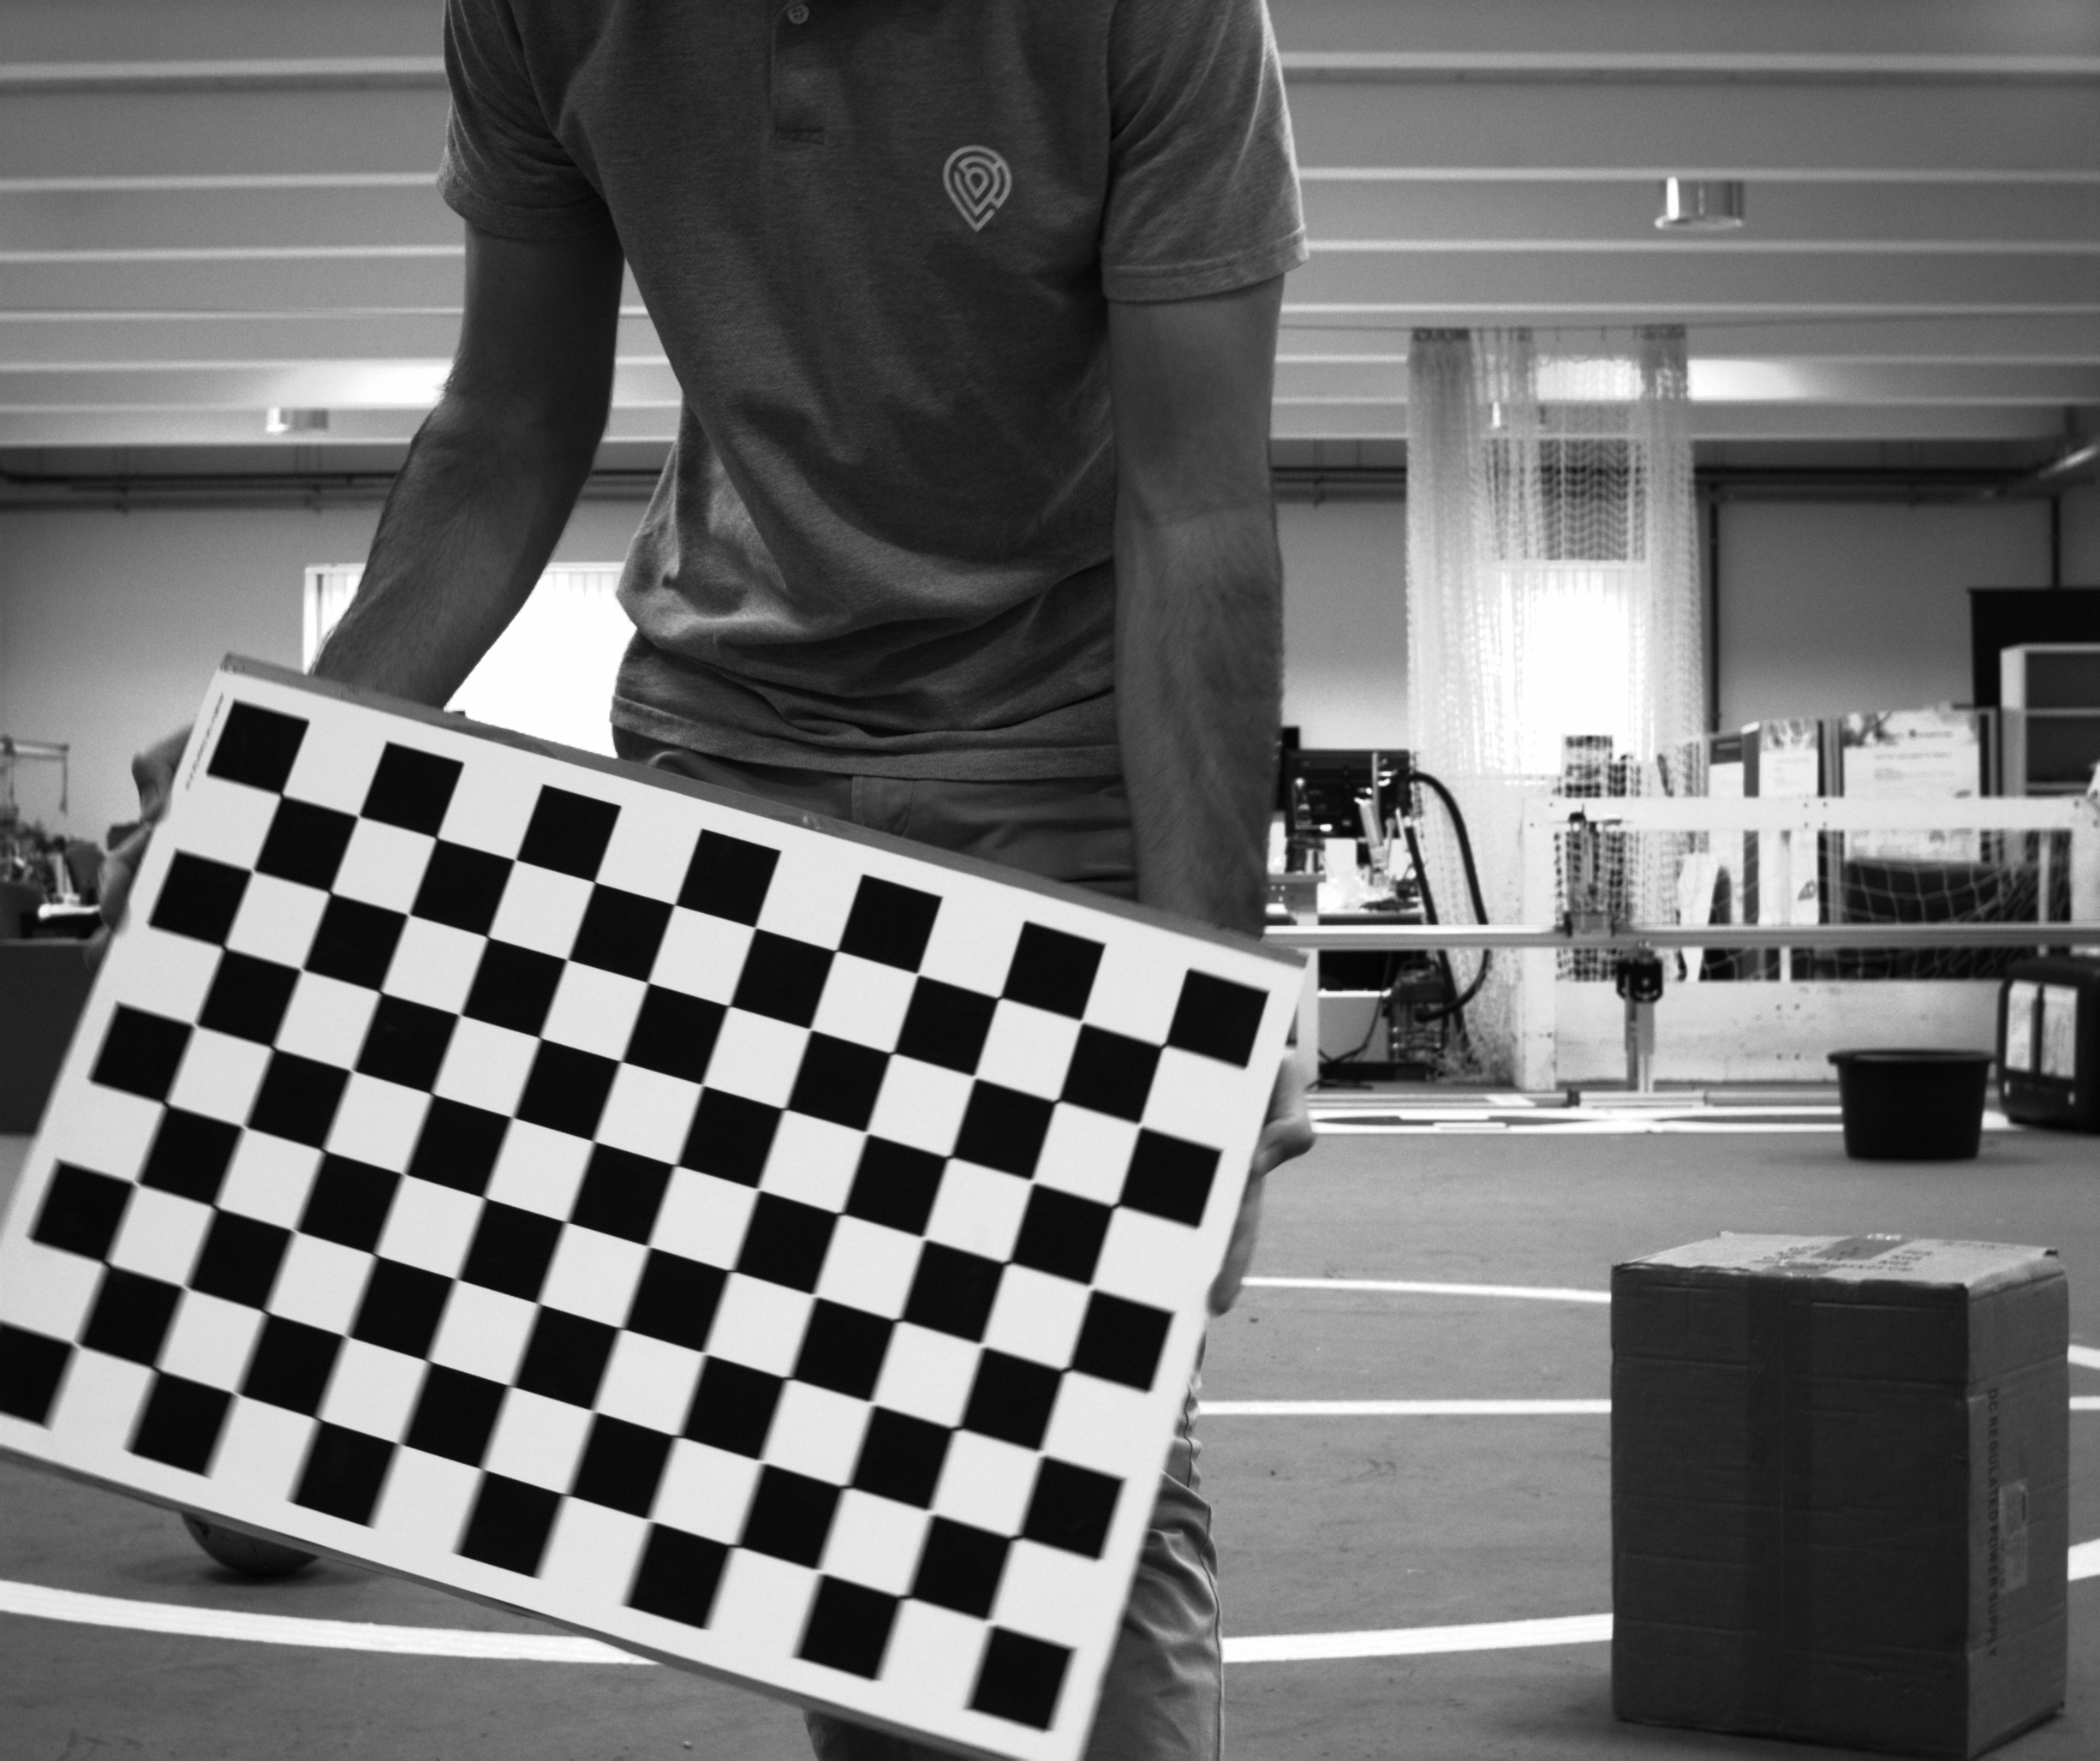
\includegraphics[width=0.9\textwidth]{img/camera-calibration/left-0044.png}
	\end{subfigure}
	\begin{subfigure}[c]{0.30\textwidth}
		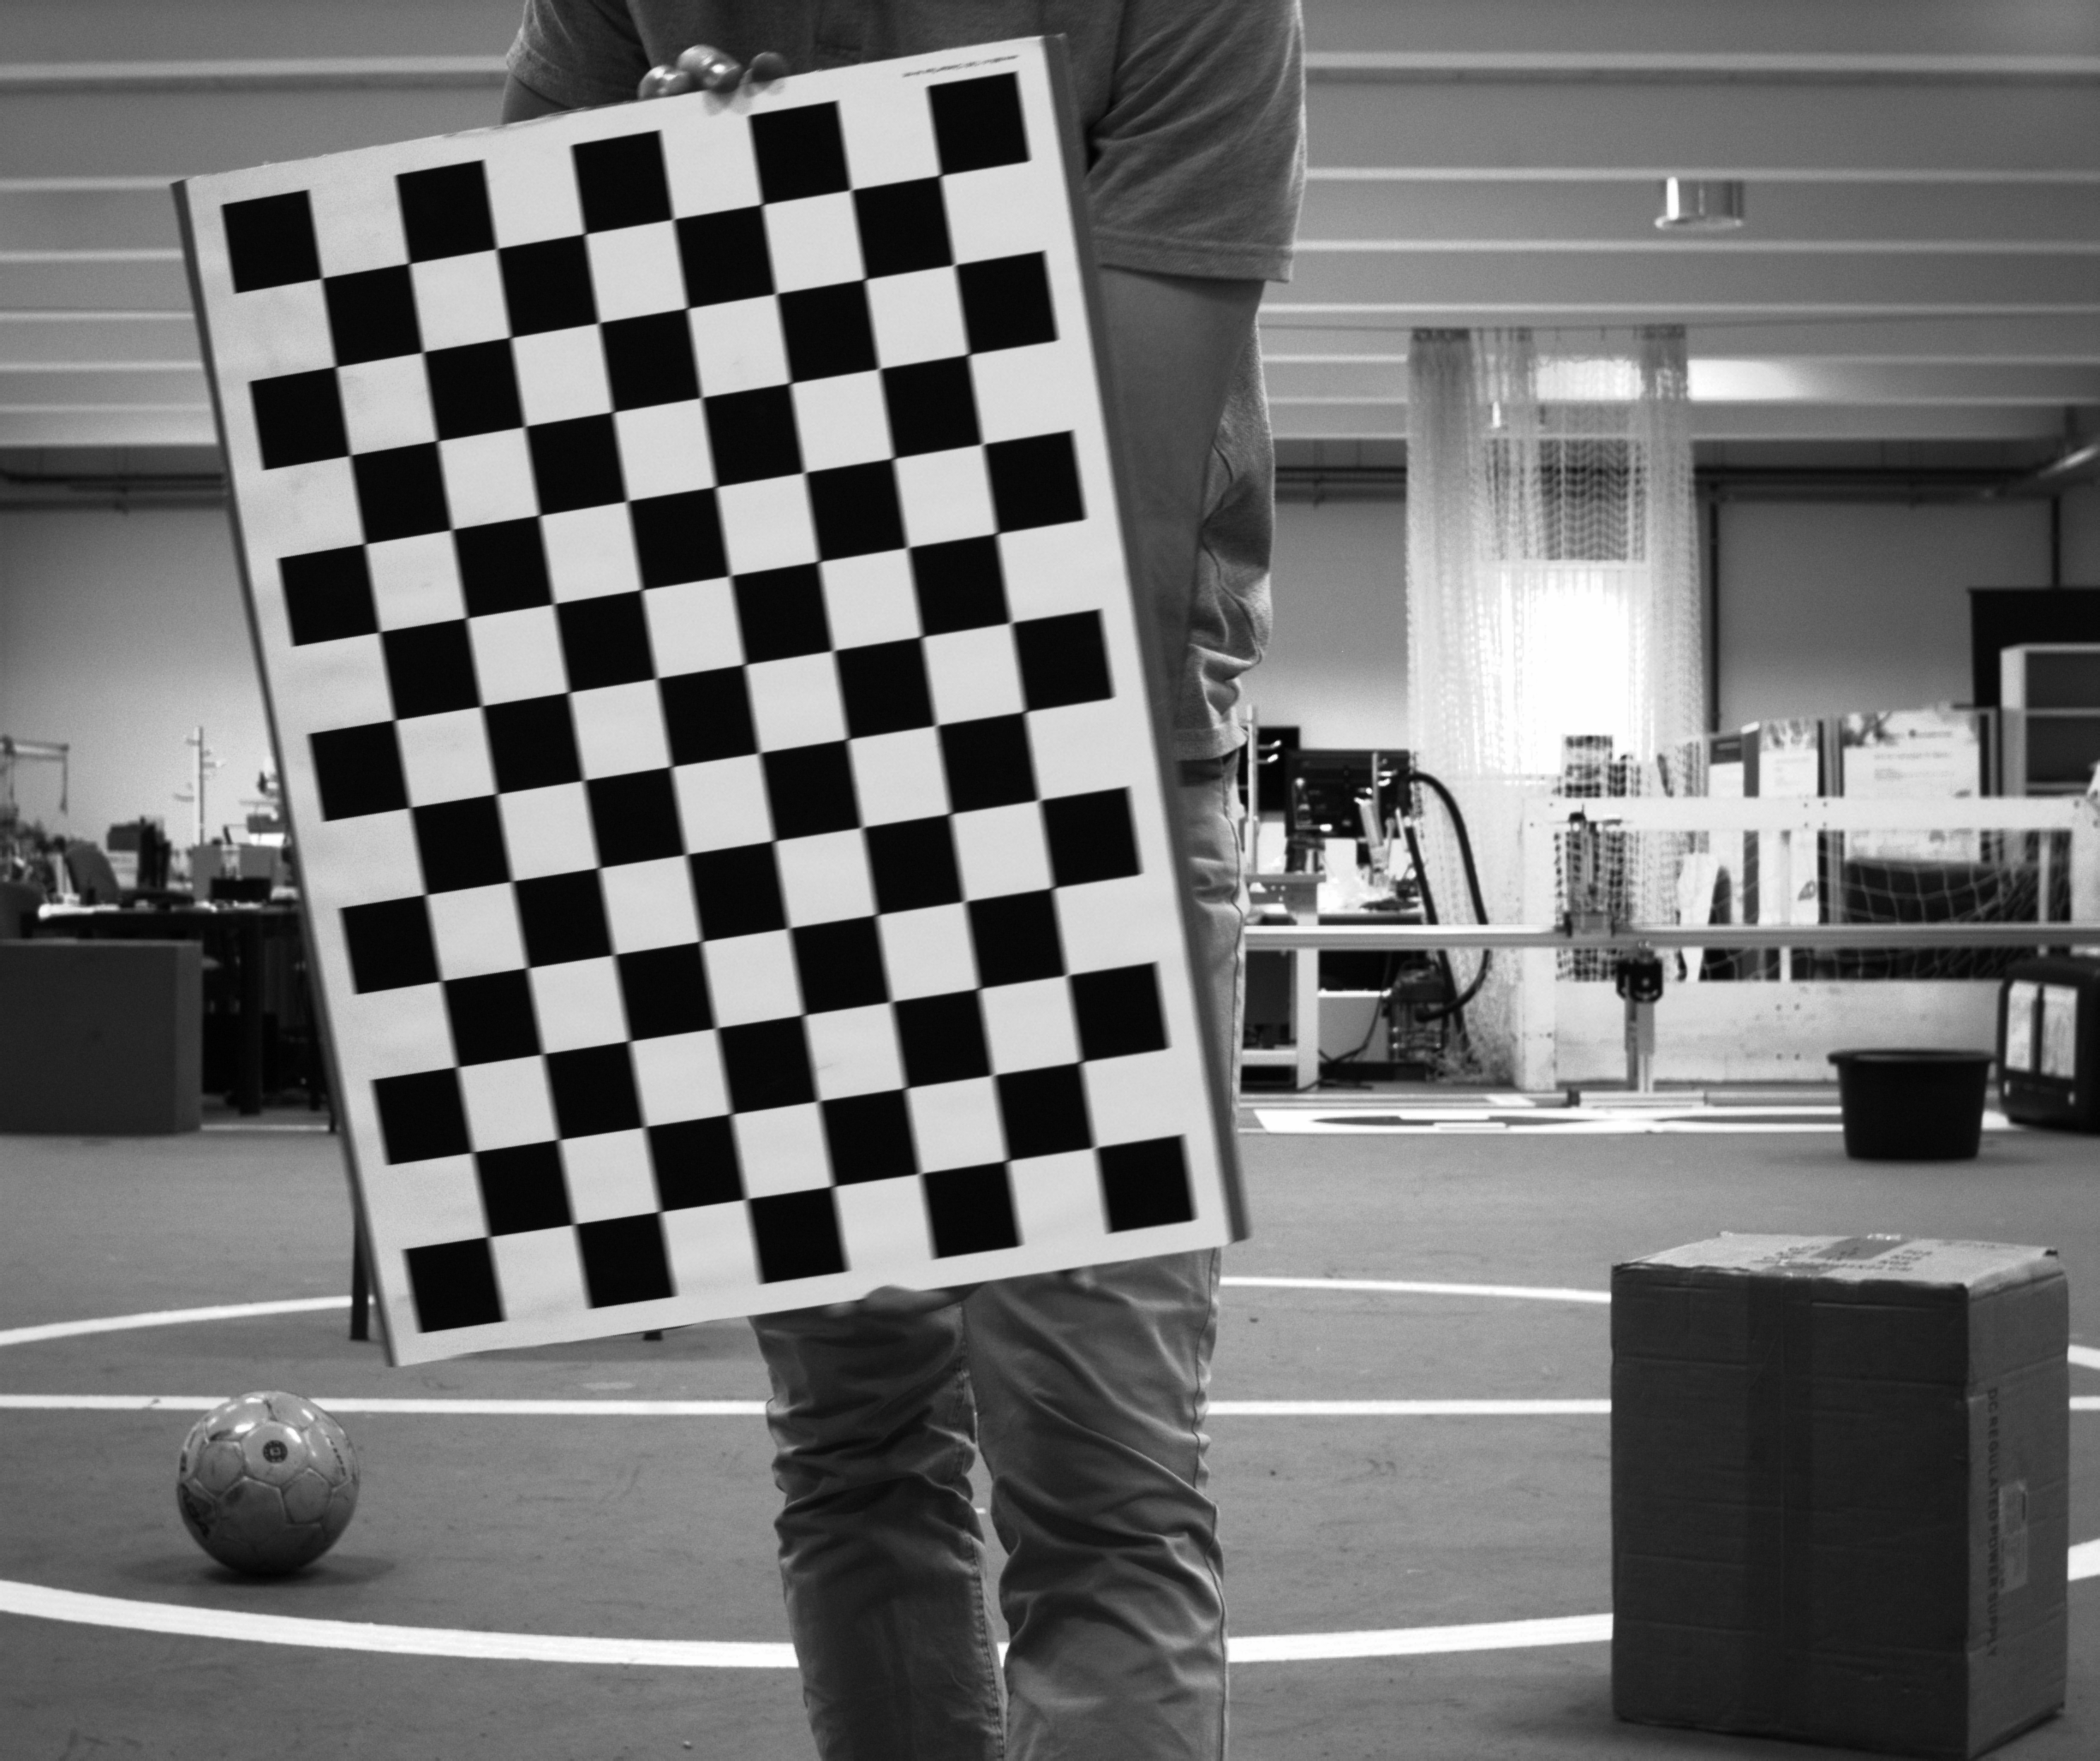
\includegraphics[width=0.9\textwidth]{img/camera-calibration/left-0048.png}
	\end{subfigure}
	
	\caption[Subset of figures used for intrinsic camera calibration.]{Subset of 6 figures used on camera intrinsic calibration. The figures are all on greyscale and for each figure, the chessboard pattern was moved to generate a unique rotational matrix and translation vector in relation to the camera coordinate frame.}
	\label{fig:camera-calibration-images}
\end{figure}

\subsubsection{Frame Rate and Bandwidth concerns}
Despite the straightforwardness of the process, one of the secondary goals of this thesis is to produce a dataset of scenarios on which \ac{lidar} interference is present. Such goal implies that all data must be properly recorded, organized and stored, including calibration data. \ac{ros} provides \texttt{rosbag}, a package for recording and playing back messages exchanged in a \ac{ros} network, which is used to save data on an external hard-drive.

However, preliminary tests with this tool indicate that it cannot save image topics at $9.2$~\ac{fps}. Other tests have shown that $8$~\ac{fps} is the best scenario where \texttt{rosbag} can record data without causing buffer flush due to overrun errors. 

When calibrating the camera, \texttt{camera\_calibration} package drops the frame rate to $\approx 4$~\ac{fps}, because it cannot operate at the desired data flow. If de-Bayerization\footnote{Converting the raw data, stored on a Bayer Filter raw format, to a RGB image} and/or rectification is being applied to the image for saving a pre-processed image, frame rate drops to $\approx 2$~\ac{fps}, since \texttt{image\_proc}, the package responsible for pre-processing the image, cannot process images at the data-rate required for them to be saved on disk, introducing an overhead. Therefore, all images are sent from camera on the raw format \texttt{BayerGB8} and recorded with \texttt{rosbag} in the same format. Note that despite the camera providing  the \texttt{RGB8Packed} color format, the hardware processing required on the camera hardware forces frame rate to be below $8$ \ac{fps}, reason why it was not chosen.

At 8~\ac{fps}, the bandwidth occupied by a 5~\ac{mp} image stream is $8 \cdot 2452 \cdot 2056 \approx \SI[per-mode=symbol]{40}{\mega\byte\per\second}$. Manta's bandwidth limit configuration register was set to a value $25\%$ higher, \SI[per-mode=symbol]{50}{\mega\byte\per\second}, to accommodate other transmissions from the computer to camera and vice-versa. No bandwidth problems were registered, besides occasionally frame drops on the starting or ending of computer processes.

Therefore, for normal operation, Manta \ac{avt} G-504C is set to trigger image capture at a fixed frame rate of $8$~\ac{fps} and when being under an internal calibration procedure, at $4$~\ac{fps}. If better computer hardware has available, internal calibration procedure could be runt at the same frame rate as normal operation, since the bottleneck is on the computer.

However, to ensure the camera runs at the desired number of \ac{fps}, other parameters that affect frame rate must also be managed, such as exposure time.


\subsubsection{Lens Aperture and Exposure Time}
Thorlabs\cp~MVL16M1 lens has several possible apertures: $f/1.4$, $f/2.0$, $f/2.8$, $f/4.0$, $f/8.0$, $f/16.0$. The smaller the F-number\footnote{F-number represents the ratio of the lens' focal length to its effective aperture diameter.}, the bigger the entrance aperture, allowing the camera sensor to be exposed to more light within the same time interval. More light indicates that exposure time can be reduced, since the sensor receives the same amount of light in less time to produce a sharp image.

However, decreasing the F-number reduces the Hyperfocal distance (see Equation~\eqref{eq:hyperfocal_distance}), which in turn reduces the \acf{dof}. A trade-off must then be addressed between \ac{dof} and F-number, which implies that three parameters must be fine-tuned: \ac{dof}, exposure time and image frame rate, since they are all interconnected. As stated above, a maximum \ac{fps} is desirable, but due to recording constraints of the \texttt{rosbag} package, $8$~\ac{fps} is the target image frame-rate. This implies that, at $8$\ac{fps}, the camera must never take more than \SI{125}{\milli\second} since the start of exposure to the broadcast of the message on the Ethernet network, which means that exposure time must be shorter. Through experimental analysis, the maximum exposure which seems to not disturb the desired frame rate is \SI{100}{\milli\second}. 

The F-number needs to be adjusted not only to ensure the requirements of the exposure time are met and to maximize \acl{dof}, but also to ensure that exposure can be increased or decrease to accommodate the daylight intensity variations. Considering a maximum exposure time of \SI{100}{\milli\second}, only aperture values greater than $f/4.0$ result on a sharp image under those constraints. To maximize the \ac{dof}, the smaller F-number should be chosen, since \ac{dof} and the F-number are inversely proportional. Therefore, with such constrains, our experimental setup uses an F-number of $f/4.0$ and an exposure time that varies between \SIrange{80}{100}{\milli\second} during daylight.

\subsubsection{\acl{dof} and calibration object}
\label{subsec:calibration:dof-and-calibration-object}
Solving Equation~\eqref{eq:hyperfocal_distance} and replacing its result on Equation~\eqref{eq:dof-subject-distance}, we can obtain $d$, the object distance at which the camera must be focused. The object to be focused is the calibrating pattern and the $DoF_{near}$ limit is select to be the distance at which the calibration pattern fills the camera~\ac{fov}. The calculations can be seen in Equation~\eqref{eq:hyperfocal-and-dof-values}.

\begin{subequations}
	\label{eq:hyperfocal-and-dof-values}
	\begin{align}
		H & = \frac{16mm^2}{4.0 \cdot 0.020mm} + 16mm  = 3.216 m \label{eq:hyperfocal-distance-value} \\
		\vspace{25mm}
		d & = \frac{(3.216 - 16mm) \cdot 1.405}{3.216 - 1.405} = 2.49m \label{eq:dof-subject-distance-value}
	\end{align}
\end{subequations}

After focusing the camera, the \texttt{cameracalibrator.py} node is run, using the command below. Note that the chessboard patterns argument is $12\times 8$ and not $13 \times 9$, because the \texttt{size} argument refers to the number of interior corners, not number of squares on the chessboard.


\begin{verbatim}
    rosrun camera_calibration cameracalibrator.py --size 12x8 --square 0.044  
        monocular:=/camera image:=/camera/image_raw
\end{verbatim}


After the \ac{gui} registers all the images, the calculation of calibration parameters can be initiated and the parameters are saved on a \textit{.ost} file for later use and/or sent the configuration to the camera. 

To interact with the Manta AVT G-504C, \texttt{avt\_vimba\_camera} \ac{ros} package~\cite{AVTROSdriver}, which depends on VIMBA GigE SDK, is used to operate the camera. It also provides compatibility with the \texttt{camera\_calibration} package, crucial for a straightforward calibration process.

\subsection{Camera Calibration Results}
The \ac{ros} node diagrams can be seen on Figure~\ref{fig:camera-calibration-rosgraph}. On sub-Figure~\ref{fig:camera-calibration-bag-rosgraph}, the nodes and topics for the calibration procedure using the data published by the \texttt{rosbag} tool. On sub-Figure~\ref{fig:camera-calibration-avt-rosgraph}, the nodes and topics for the calibration procedure using the data directly from the driver are shown. 


\begin{figure}[H]
	\vspace{5mm}
	\centering
	\begin{subfigure}[c]{0.8\textwidth}
		\centering
		\def\svgwidth{\columnwidth}
		\graphicspath{{img/camera-calibration/}}
		\includesvg{img/camera-calibration/bag-rosgraph}
		%
\includegraphics[width=0.8\textwidth]{img/camera-calibration/bag-rosgraph.png}
		\caption{\ac{ros} node graph for the camera calibration procedure using the \texttt{rosbag} tool. \texttt{RosbagPlayer} is the node that plays back the data stored on the bag file.}
		\label{fig:camera-calibration-bag-rosgraph}
	\end{subfigure}
	\vspace{5mm} \\ 
	\begin{subfigure}[c]{0.8\textwidth}
		\centering
		\def\svgwidth{\columnwidth}
		\graphicspath{{img/camera-calibration/}}
		\includesvg{img/camera-calibration/avt-rosgraph}
		%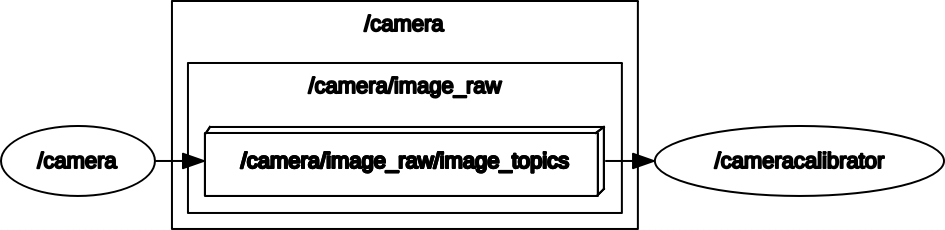
\includegraphics[width=0.8\textwidth]{img/camera-calibration/avt-rosgraph.png}		
		\caption{\ac{ros} node for the camera calibration procedure using the \ac{avt} Vimba \ac{ros} driver. \texttt{camera} node refers to \ac{ros} node that wraps the \ac{avt} Vimba driver.}
		\label{fig:camera-calibration-avt-rosgraph}
	\end{subfigure}
	\caption[Camera calibration \acs{ros} node diagram.]{Camera Calibration node graph for \ac{ros} nodes. \texttt{cameracalibrator} is the node responsible for computing the intrinsic camera calibration parameters, either if they are (\subref{fig:camera-calibration-bag-rosgraph}) being replayed using \texttt{rosbag}; (\subref{fig:camera-calibration-avt-rosgraph}) or coming directly from the camera driver.}
	\label{fig:camera-calibration-rosgraph}
\end{figure}

The camera was calibrated daily whenever experimental measures were taken. The calibration for one of these days is shown below, where $\mathbf{K}$ is the camera intrinsic parameters' matrix, $\mathbf{D}$ is the lens distortion coefficients vector and $\mathbf{P}$ the camera projective matrix. %on Equation~\eqref{eq:camera-calibration-results}.

\begin{subequations}
	\label{eq:camera-calibration-results}
	\begin{align}
		\mathbf{K} & = 
		\begin{bmatrix}
			4595.944192 & 0.0         &  1313.9194945 \\
			0.0         & 4593.466666 &  952.554450 \\
			0.0         & 0.0         &  1.0
		\end{bmatrix} \nonumber \\
		\mathbf{D} & = 
		\begin{bmatrix}
			-0.304037 & 1.364428 &  -0.005705 & 0.003330 & 0.0
		\end{bmatrix} \nonumber \\
		\mathbf{P} & = 
		\begin{bmatrix}
			4529.381836 & 0.0         & 1318.010062 & 0.0 \\
			0.0         & 4534.939941 & 947.167736  & 0.0 \\
			0.0         & 0.0         & 1.0         & 0.0 
		\end{bmatrix}
		\nonumber
	\end{align}
\end{subequations}

	

\section{\ac{lidar} Intrinsic Calibration}
Unlike a camera, \acp{lidar} do not possess a typical calibration procedure. For Velodyne VLP-16 reflectivity measurements are factory calibrated, in a procedure described in~\cite{vlp16} and a \ac{xml} file is provided with the \ac{lidar}, containing corrections for the \ac{lidar} operating parameters.

This file must be converted to a more suitable format, \acs{yaml}~\footnote{\acs{yaml} is an acronym for \acl{yaml}. The author chose not to follow the norm of expanding acronyms' inline due to acronym recursive nature, to facilitate reading.}, which is \ac{ros} default and can be loaded by the Velodyne \ac{ros} driver package, \texttt{velodyne}, for correction of the \ac{lidar} measurements. After observing the point cloud with test objects such as boxes and walls, \ac{lidar} calibration is observed to be accurate and no further calibration procedures were undertaken.

\section{Camera and \ac{lidar} Extrinsic Calibration}
\label{sec:calibration:extrinsic}
Calibrating the camera and \ac{lidar}, as explained in Section~\ref{subsec:sota:camera-intrinisc-calibration}, requires determining the rigid body transform between the reference frames of the two sensors. A rigid body transform, also known as a Euclidean Isometry since it preserves the distance between points~\cite{mvg_book}, has 6 degrees of freedom, that can be represented by a translation and a rotation vector.

Due to the ambiguity of the rotation vector and its variety of interpretations: (1) it can represent one of twelve Euler angles notation, angle axis notation, amongst others; (2) this notation is normally replaced by the unambiguous rotation matrix (see Equation~\eqref{eq:camera_transform_full} for an example) or a quaternion. Such representations are also free from gimbal lock, a mathematical limitation of the vector representation, that can cause one rotation axis ``locking'' on another, resulting on their rotation no longer being independent of the other, removing one \acl{degof} and degenerating into a two-dimensional rotational space. For more details on gimbal lock and other singularities see~\cite{mvg_book, Slabaugh, camera_models}.

In this thesis, the preferred notation is a quaternion, which is also adopted by \ac{ros}~\cite{Foote2014}. A quaternion is a mathematical object belonging to $\mathbb{R}^4$, that has a vector (or imaginary) part and a scalar (or real) part. Its representation is denoted on Equation~\eqref{eq:quaternion-notation}, where $\mathbf{i}$, $\mathbf{j}$ and $\mathbf{k}$ are the normalized unit vectors of the $x$, $y$ and $z$ axis, respectively; and $w$ is the scalar part. More information on quaternions can be found on~\cite{mvg_book}.

\begin{equation}
	\label{eq:quaternion-notation}
	q = (x\mathbf{i}, y\mathbf{j}, z\mathbf{k}, w)
\end{equation}

\subsection{Calibration Method}
\label{subsec:calibration:calibration-method}
Given the nature of the sensors: a camera image is two-dimensional and the \ac{lidar} data is tridimensional; the extrinsic calibration needs to consider the projective geometry and its transformations on the camera. Revisiting Equation~\eqref{eq:jointRotationTranslationTransform}, our goal is to determine the joint rotation and translation matrix that allows the conversion of coordinates from the \ac{lidar} to the camera frame. To account for projective geometry, Equation~\eqref{eq:camera_transform_full} must be considered when establishing 3D points to image pixels correspondences.

The method implemented to calibrate the camera and \ac{lidar} is inspired by Scaramuzza's\etal~\cite{Scaramuzza} and Brabec's~\cite{brabec2014} work. The method proposed consists on manually selecting the correspondences between image pixels and 3D points on the \ac{lidar} point cloud. If a single synchronized frame from the camera and \ac{lidar} is used, one can consider the scene as static, and therefore, the joint rotation and translation matrix present in Equation~\eqref{eq:camera_transform_full} is actually the same as the matrix present on Equation~\eqref{eq:jointRotationTranslationTransform}. 

Such considerations are only possible due to the camera using a global shutter instead of rolling shutter. In the former, the image is acquired in a single shot and all the points ``have the same timestamps''. In the latter, each row of the image is acquired one after another, iteratively, therefore, ``having different timestamps''. If a rolling shutter camera was used, for a single image, the \ac{lidar} point cloud could not have been considered static and the delays on the camera shutter and \ac{lidar} rotation would have to be taken into account when calibrating and fusing the data between the two. An exception to the latter is if the \ac{lidar} and camera position is static and the scene is also static.

Since the intrinsic calibration matrix is already obtained by the method described on Section~\ref{sec:calibration:camera}, and the correspondences are selected by the user, the only remaining unknown is the joint rotation and translation matrix. Also, since this method ``reuses'' the equations that are the basis for intrinsic camera calibration, it can also ``reuse'', with some constraints and modifications, the same algorithms~\cite{opencv_doc}, such as \texttt{solvePnP}, which determines the joint rotation and translation matrix that converts world points to camera pixels.


\subsection{Implementation}
To extrinsically calibrate the camera and \ac{lidar}, a multi-node network approach was followed, which can be seen on Figure~\ref{fig:extrinsic-calibration-rosgraph}. Using \ac{opencv} and \ac{pcl}, two visualizers were encapsulated under \ac{ros} nodes written in C++, that subscribe camera and \ac{lidar} messages, respectively. The point cloud visualizer, \texttt{PCL\_Viewer\_with\_Pose}, receives the point cloud data from the \texttt{rosbag} player or the \texttt{velodyne} driver and publishes the coordinates of the selected point and the viewer pose. \texttt{Image\_Visualizer} publishes the pixels selected by the user, but requires the de-Bayering and conversion to RGB of the raw image using the \texttt{image\_proc} package. Despite being wrapped in \ac{ros}, each of the visualizers provides standalone callbacks, that support ``frame freezing'' for correspondences selection.

Another node, \texttt{rigid\_transform\_computation} is responsible for listening to messages containing the selected pixels and points, registering their correspondences. This node  instantiates two \ac{ros} services servers, that can be called asynchronously: one for computing the rigid body transform and another to save the correspondences selected on a \ac{csv} file, for later usage. 

\begin{figure}[!ht]
	\centering
	\def\svgwidth{\columnwidth}
	\graphicspath{{img/calibration/}}
	\includesvg{img/calibration/extrinsic-calibration-rosgraph}
	\caption{\ac{ros} node graph for the extrinsic calibration. The nodes are represented in  ellipses and the topics between them in rectangles. Rosbag Player is responsible reproducing the recorded topics.}
	\label{fig:extrinsic-calibration-rosgraph}
\end{figure}


The algorithm implemented to compute the 6-\ac{degof} rigid body transformation uses \ac{opencv} \texttt{solvePnP}, which gives the intrinsic camera parameters and the manually selected correspondences between the object points (3D points from \ac{lidar}). It can also compute the rotation and translation vectors. For solving the \ac{pnp} problem, several algorithms can be used: Levenberg-Marquardt~\cite{Levenberg1943}, Effective~\ac{pnp}~\cite{Lepetit2009}, Perspective-Three-Point~\cite{Gao2003}, Direct-Least-Squares~\cite{Hesch2011} or Exhaustive Linearization — Uncalibrated \ac{pnp}~\cite{Penate-Sanchez2013a}. The \ac{ros} node implemented provides an argument to select the desired algorithm to be applied to solve the \ac{pnp} problem.

After resolving the \ac{pnp} with one of the methods above, Rodrigues' algorithm is used to convert the \ac{opencv} rotation vector to a rotation matrix~\cite{Dai2015}, which is then used to derive the quaternion. Combining the quaternion with the translation vector, a static transform is published to the \ac{ros} network, which can be used to convert and fuse data from the camera coordinate frame to the \ac{lidar} and vice-versa.

An additional \ac{ros} node is also created to compute and publish the rigid body transformation from pre-selected correspondences. It loads the correspondences between the 3D points and image pixels from the \ac{csv} file, the camera intrinsic parameters from an \acs{yaml} file. Using the same algorithms as \texttt{rigid\_transform\_computation}, it computes the rigid body transform and publishes it to the \ac{ros} network using \ac{ros} static transformation.


\subsection{Calibration Result}
\label{subsec:calibration:extrinsic-results}
To ease the calibration process, a \ac{ros} launch file is created. A launch file is written in \ac{xml} and provides instructions to \ac{ros} master node on how to run all the necessary nodes to implement a desired functionality. On this case, \texttt{rigid\_transform\_computation.launch}, launches the two visualizers (image and point cloud) and the node responsible for listening to the selected correspondences. 

Several tests were performed with the possible algorithms for solving \ac{pnp}. Since for the version of \ac{opencv} used, $3.2.0$, the Direct-Least-Squares and Uncalibrated \ac{pnp} methods are unstable~\cite{opencv_doc}, with only the Levenberg-Marquardt, Perspective-Three-Point and Effective~\ac{pnp} were tested. 

Although the planar chessboard used for intrinsic camera calibration was present during the extrinsic calibration, the algorithm implemented does not require the usage of a calibration object. For calibration, 6 points were selected in the point cloud and 6 pixels on the image: four of them correspond to the corners of the chessboard and two to a background object. The selected correspondences can be seen in Figure~\ref{fig:calibration-correspondences}: sub Figure~(\subref{fig:extrinsic-calibration-correspondences:camera}) shows the selected pixels on the image, marked with red crosses; sub Figure~(\subref{fig:extrinsic-calibration-correspondences:lidar}) shows the selected 3D points on the point cloud, marked as red spheres.


\begin{figure}[H]
	\centering
	\begin{subfigure}[c]{0.39\textwidth}
		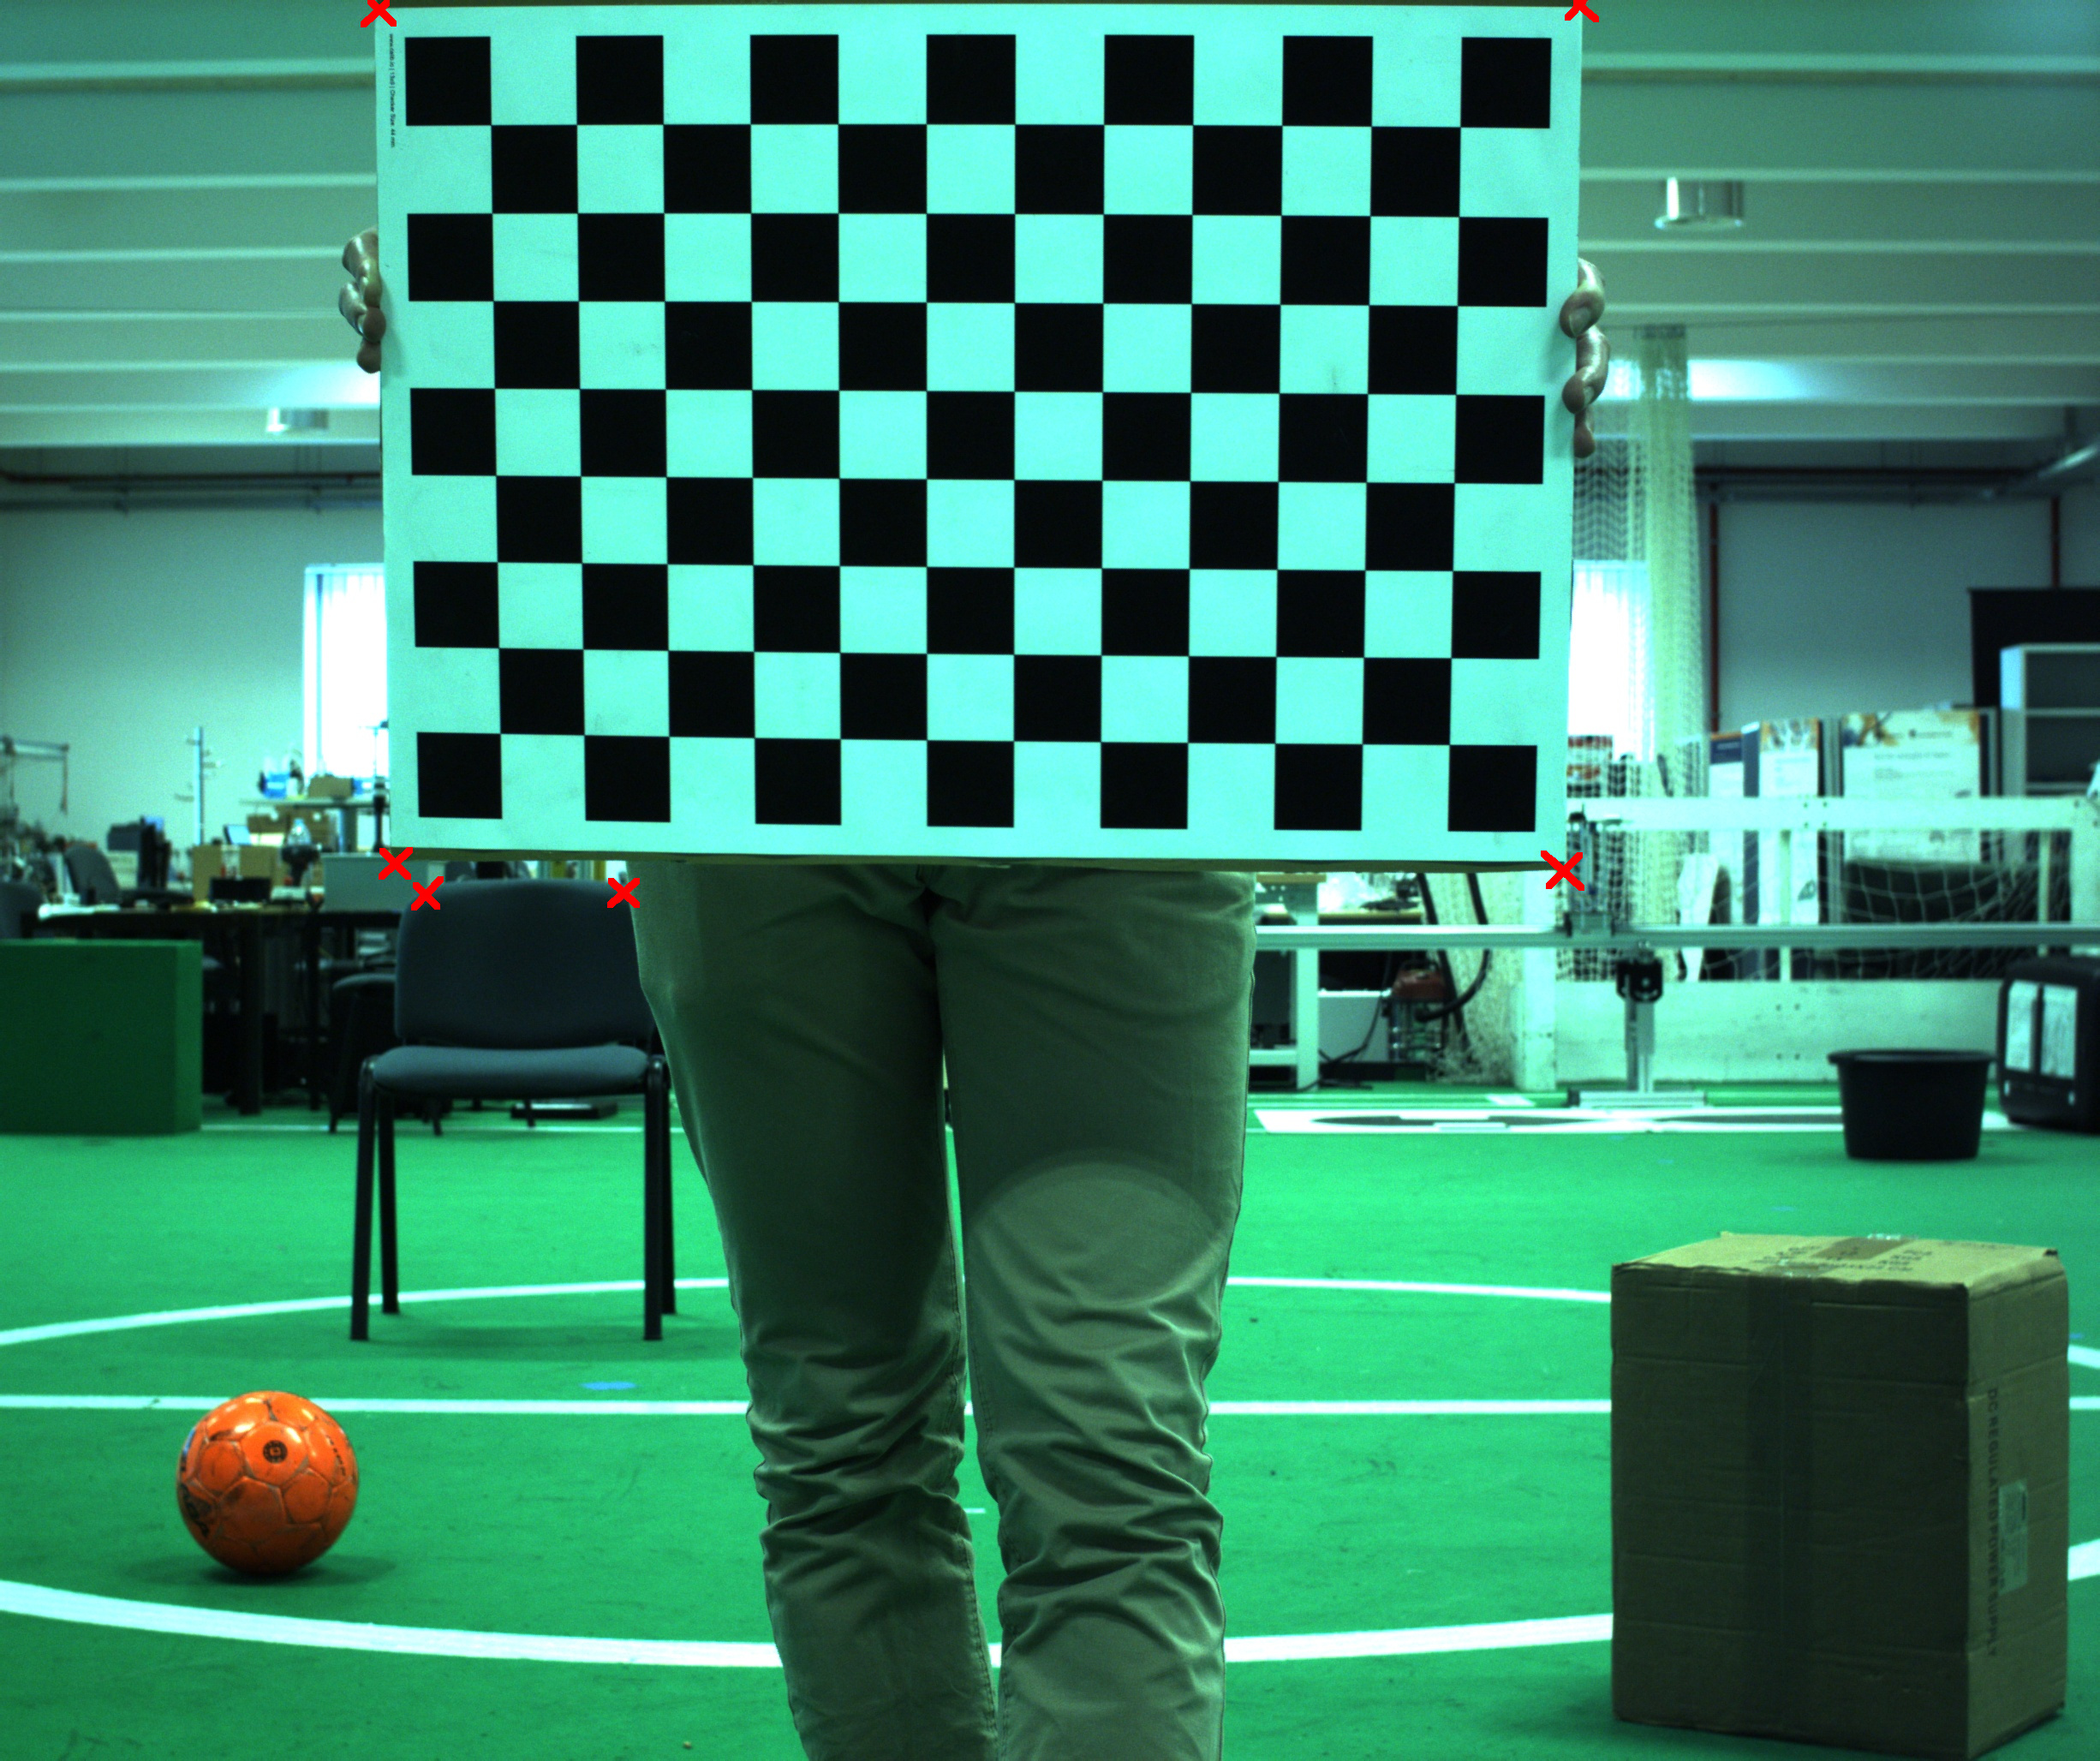
\includegraphics[width=\textwidth]{img/calibration/camera-extrinsic-calibration-points-draw.jpg}
		\caption{}
		\label{fig:extrinsic-calibration-correspondences:camera}
	\end{subfigure}
	\qquad
	\begin{subfigure}[c]{0.55\textwidth}
		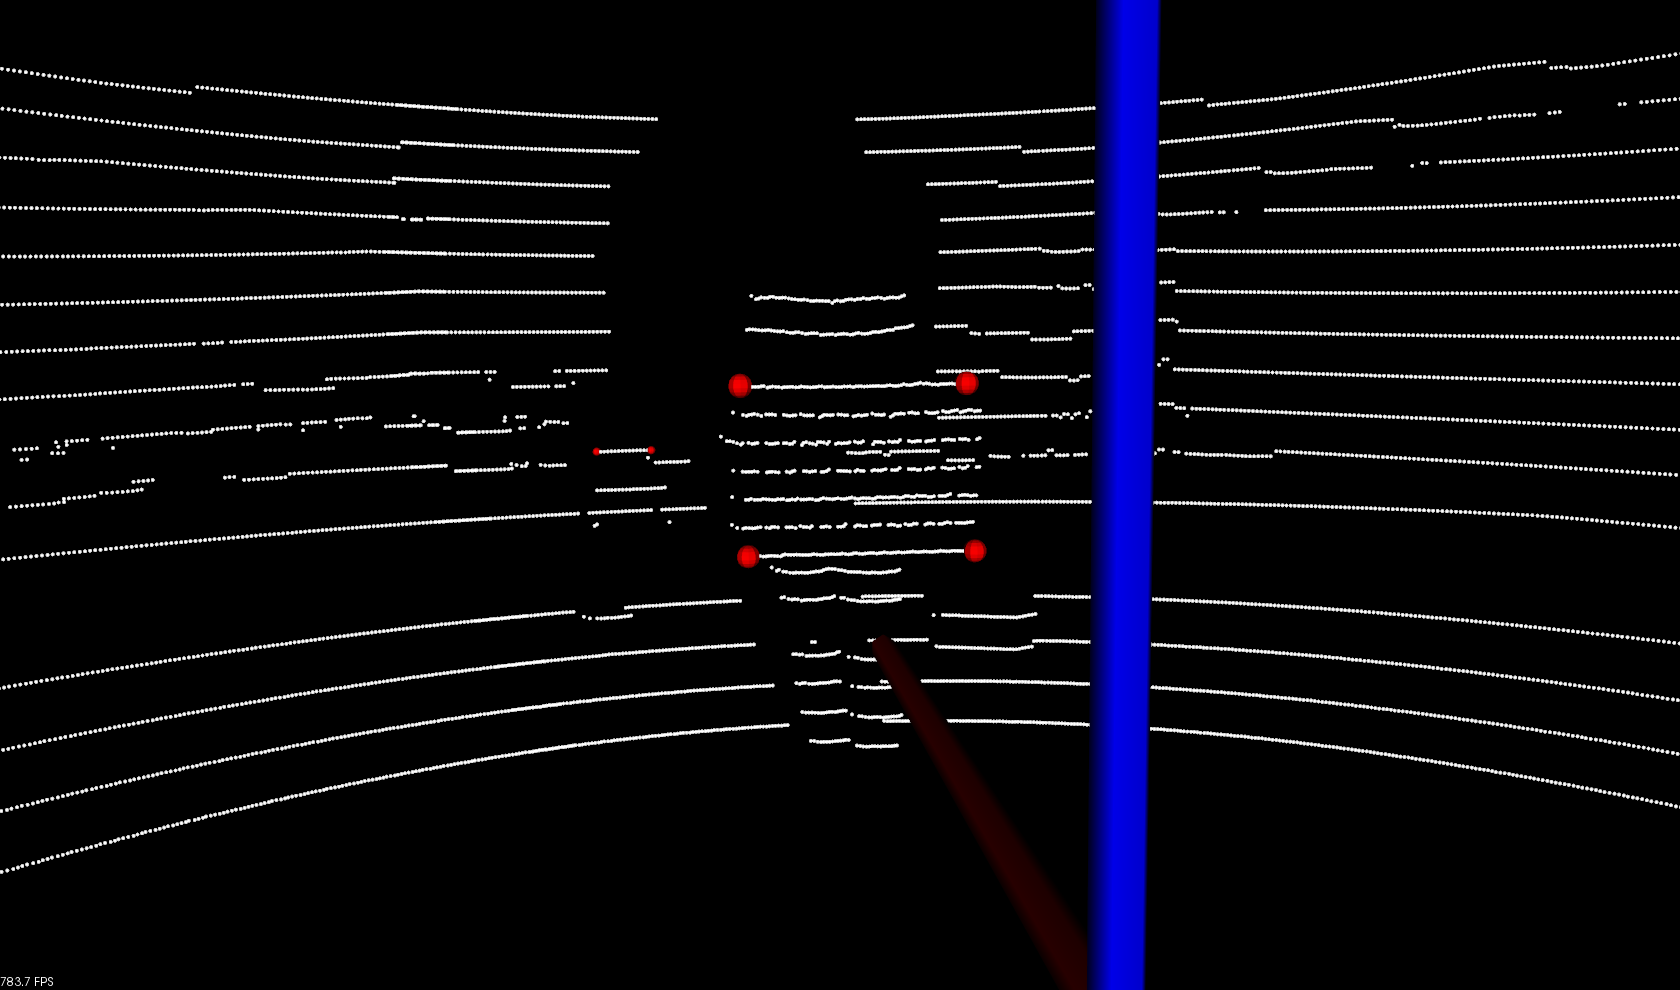
\includegraphics[width=\textwidth]{img/calibration/lidar-extrinsic-calibration-points.png}
		\caption{}
		\label{fig:extrinsic-calibration-correspondences:lidar}
	\end{subfigure}
	\caption[Correspondences selected on the image and point cloud for extrinsic calibration between the two.]{Image~(\subref{fig:extrinsic-calibration-correspondences:camera}) and Region of the Point Cloud~(\subref{fig:extrinsic-calibration-correspondences:lidar}) used on the extrinsically calibration between the camera and the \ac{lidar}. The correspondences are marked with red crosses or spheres, respectively, and correspond to the 4 corners of the chessboard and the limit of the chair on the background.}
	\label{fig:calibration-correspondences}
\end{figure}

After the manual selection of the points, the rotation and translation are obtained from the camera frame to the \ac{lidar} frame. If the transformation from the \ac{lidar} to the camera frame is required, the inverse transformation can be obtained by inverting the scalar component of the quaternion, $w$, as depicted in Equation~\eqref{eq:quaternion-inversion}. 

\begin{equation}
	\label{eq:quaternion-inversion}
	w^\text{LiDAR}_\text{camera} = - w^\text{camera}_\text{LiDAR}
\end{equation}

Extrinsic camera and \ac{lidar} calibration was performed whenever experimental measures were taken. The calibration for the camera intrinsic parameters given on Equation~\eqref{eq:camera-calibration-results} and the correspondences shown on Figure~\ref{fig:calibration-correspondences} are presented on below. On Figure~\ref{fig:extrinsic-calibration-frames}, a visualization of the experimental setup sensors coordinate frames and the transformation between them is given.

\begin{subequations}
	\label{eq:camera-to-lidar-transform}
	\begin{align}
		t = \begin{bmatrix}
			-0.156714088124  \\
			-0.0206731034739 \\
			-0.258170823407
		\end{bmatrix} \nonumber
		& \qquad
		q = \begin{bmatrix} 
		 0.4872192 \\
		-0.4999094 \\
		 0.5216904 \\
		-0.4904560
	\end{bmatrix} \nonumber
	\end{align}
\end{subequations}

\begin{figure}[H]
	\centering
	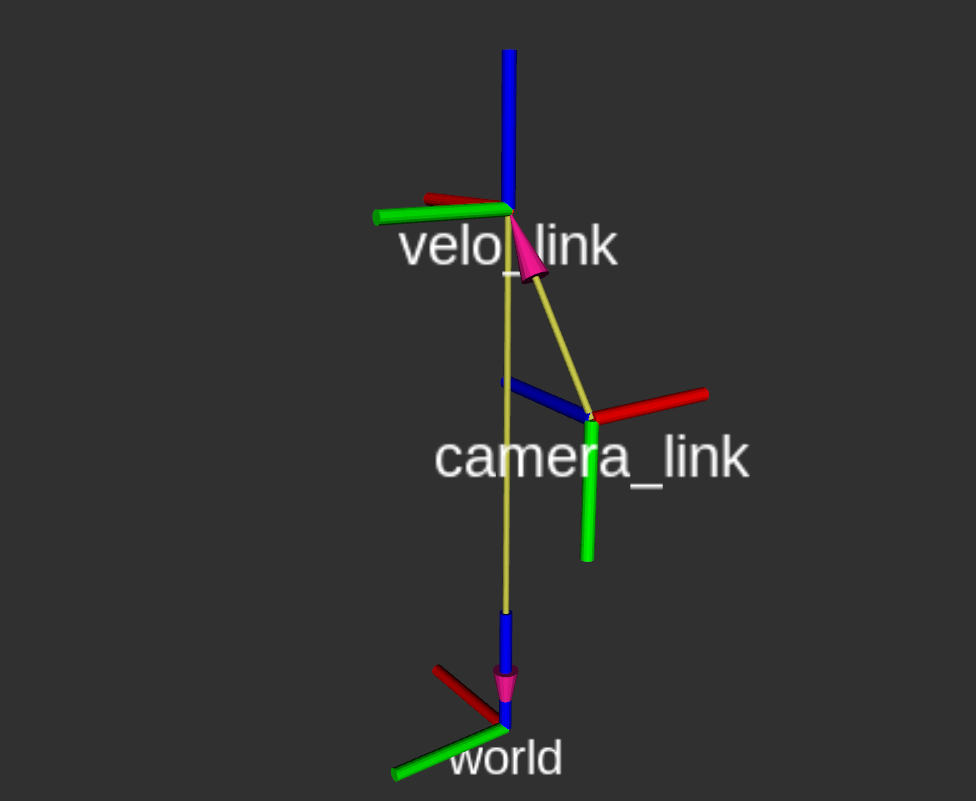
\includegraphics[width=0.5\textwidth]{img/calibration/extrinsic-calibration-frames.png}
	\caption[Experimental setup TF tree coordinate frames.]{TF visualization on \texttt{Rviz} of the TF tree between the experimental setup coordinate frames. \texttt{velo\_link} and \texttt{camera\_link} represent the coordinate frames of the Velodyne VLP-16 \ac{lidar} and the Manta \ac{avt} G-504C, respectively. The \texttt{world} coordinate frame represents the positioning of the \ac{lidar} in the world, which in this case is an offset to the vertical positioning of the \ac{lidar}.}
	\label{fig:extrinsic-calibration-frames}
\end{figure}

\subsection{Comparison with \ac{kitti}}
\label{subsec:calibration:kitti-comparision}

On \ac{kitti}, the number of coordinate frames is greater and have more complex interactions. While on the experimental setup the coordinates frames are all fixed, on \ac{kitti}, there is only one fixed frame, \texttt{world}. The car coordinate frame is named \texttt{base\_link} and the transformation between the \texttt{base\_link} and the camera are time-dependent.

On the car, every sensor has a coordinate frame, that is referred to the \texttt{base\_link} referential. From all the coordinate frames, that can be seen on~\cite{Geiger2013a}, the required during this research are:

\begin{itemize}
	\item \texttt{velo\_link}: Velodyne HDL-64E \ac{lidar} coordinate frame;
	\item \texttt{camera\_color\_left}: coordinate frame of the RGB camera selected for this research;
	\item \texttt{imu\_link}: \ac{imu} coordinate frame;
	\item \texttt{base\_link}: car coordinate frame.
\end{itemize}

Comparing with our experimental setup, the \ac{lidar} coordinate frame is equal in name and the coordinate axis orientation. The camera frame only differs in their name (the coordinate axis orientation is similar). Our experimental setup do not contain an \ac{imu}, therefore there is no need for a \texttt{imu\_link}. 

Due to the experimental setup being static, the \ac{lidar} and its \texttt{velo\_link} coordinate frame is referred directly to the \texttt{world} frame with a static transforms. Since the setup does not move, there is no need for a \texttt{base\_link} frame, since it will always coincide with the world frame, because the scene is static. On Figure~\ref{fig:kitti-tf-frames}, a subset of \ac{kitti}'s coordinate frames is presented. The \texttt{world} coordinate frame is not visible on the figure. 

\begin{figure}[!ht]
	\centering
	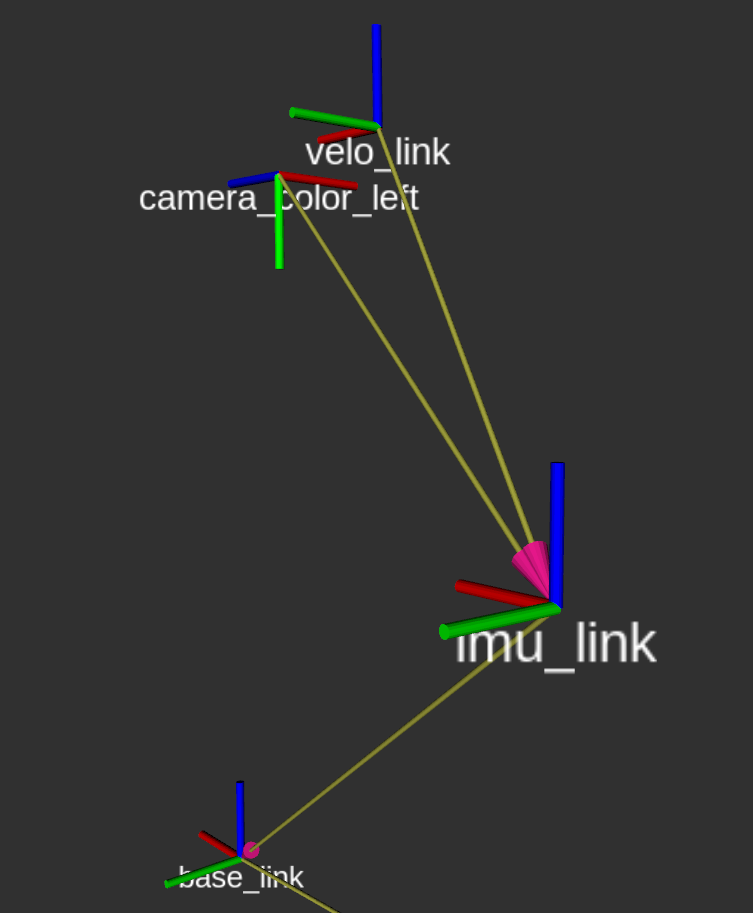
\includegraphics[width=0.5\textwidth]{img/KITTI/tf.png}
	\caption[Relevant \acs{kitti} TF tree coordinate frames.]{TF visualization on \texttt{Rviz} of the TF tree between a subset of \ac{kitti}'s setup coordinate frames. \texttt{velo\_link} and \texttt{camera\_color\_left} represent the coordinate frames of the Velodyne HDL-64E \ac{lidar} and the RGB left camera, respectively.}
	\label{fig:kitti-tf-frames}
\end{figure}

\section{Final Remarks}
\label{sec:calibration:final-remarks}

On this chapter, the experimental setup is presented and the intrinsic and extrinsic calibration of its sensors is detailed. Camera, \ac{lidar} and lens specifications are given and briefly discussed, along with their relative positioning, network setup and connection with the computer. Since camera will be used to understand and possibly mitigate \ac{lidar} interference through sensor fusion, we confirm that the camera is free from interference by the \ac{lidar} in a test without any other light sources.

Sensory calibration is performed to allow data acquisition from the camera and \ac{lidar} to construct the experimental setup dataset. Intrinsic camera calibration is carried by using \ac{ros} \texttt{camera\_calibrator.py} package and moving a chessboard in front of the camera, combining rotation and translation motions. Using Effective \acl{pnp}, the camera intrinsic matrix and the distortion coefficients for the lens are determined, which are used to rectify the camera image. Regarding \ac{lidar} calibration, the device comes calibrated by the manufacturer and only azimuthal and polar angle coefficients need to be loaded by the firmware and driver for measurement correction.

Extrinsic calibration between the camera and \ac{lidar} is performed to the determinate the rigid body transformation between the two, allowing the conversion of data between their coordinate frames. Our proposed algorithm is based on the selection of at least four $2D \leftrightarrow 3D$ correspondences between the image and the point cloud. A calibration pattern is not required. We adapt the work of Scaramuzza\etal and Brabec's, which is used to calibrate a camera, to determine the rigid body transform between the \ac{lidar} and camera, by solving for the joint rotation and translation matrix. To do so, our implementation consists of an image and point cloud visualizers, a node to receive the selected points and compute the rigid body transform and a client node to trigger the computation and saving of results.

From this chapter, our main takeout is a generic extrinsic calibration algorithm and its implementation on \ac{ros}, that can calibrated any \ac{ros} compatible monocular camera and 3D \ac{lidar}. We also intrinsically calibrate the camera, performing the first step of any computer vision project and obtain the rigid body transform between the sensors of our setup, to be used later. The work developed on this chapter is essential for the data fusion between the camera and \ac{lidar} (Chapter~\ref{chapter:sensor-fusion}) and object detection on image and estimating the correspondent bounding boxes on the point cloud (Chapter~\ref{chapter:object-detection}).
